% !TEX TS-program = pdflatex


%\documentclass[actinf,draft]{svjour}
\documentclass[smallcondensed]{svjour3}
\smartqed  % flush right qed marks, e.g. at end of proof

\usepackage{etex}

\usepackage[T1]{fontenc}
% \usepackage{geometry}                % See geometry.pdf to learn the layout options. There are lots.
%\geometry{a4paper}                   % ... or a4paper or a5paper or ...
%\geometry{landscape}                % Activate for for rotated page geometry
%\usepackage[parfill]{parskip}    % Activate to begin paragraphs with an empty line rather than an indent


%%\usepackage{graphicx}

%\usepackage{amsfonts}
%\usepackage{fancyhdr}
%\usepackage{cite}
%\usepackage{ifthen}
%\usepackage{amssymb}
%\usepackage{fancyhdr}
%\usepackage{pifont}
\usepackage{stmaryrd}
\usepackage{mathtools,mathpartir}
\usepackage{proof}
%\usepackage{setspace}
\usepackage{enumitem}
\setlist{nolistsep}
%\usepackage{indentfirst}
%%%\usepackage{amsmath,amssymb,amscd,mathrsfs}
% \usepackage{array,booktabs,arydshln,xcolor}
%
\usepackage{array,booktabs}
%\DeclareGraphicsRule{.tif}{png}{.png}{`convert #1 `dirname #1`/`basename #1 .tif`.png}
%\usepackage{epsfig,color,enumitem}
\usepackage{epsfig,enumitem}
%% \usepackage[%
%%     font={small,sf},
%%     labelfont=bf,
%%     format=hang,    
%%     format=plain,
%%     margin=0pt,
%%     %% width=0.8\textwidth,
%%     aboveskip=4pt,
%%     belowskip=-18pt,
%% ]{caption}
%% \usepackage[list=true]{subcaption}

\usepackage{soul}               % Highlighting: \hl, \so, \ul

\soulregister{\st}{8}
\soulregister\cite7
\soulregister\citep7
\soulregister\secn7
\soulregister\ref7
\soulregister\pageref7
\soulregister{\em}{0}
\soulregister{\bf}{0}
\soulregister{\fig}{7}
\soulregister{\ie}{0}
\soulregister{\etc}{0}
\soulregister{\eg}{0}
\soulregister{\wrt}{0}
\soulregister{\resp}{0}
\soulregister{\cf}{0}
\soulregister{\mdash}{0}
\soulregister{\ndash}{0}

\usepackage[colorinlistoftodos,bordercolor=white]{todonotes}
%% \usepackage[disable,colorinlistoftodos,bordercolor=white]{todonotes}

\newcommand{\noteSB}[2][color=green!40, size=\tiny]{\todo[#1]{{\bf
      Note: } {#2}}}
\newcommand{\noteEM}[2][color=blue!40, size=\tiny]{\todo[#1]{{\bf Eric: } {#2}}}
\newcommand{\noteInSB}[2][inline,color=green!40]{\todo[#1]{{\bf Simon: } {#2}}}
\newcommand{\noteInEM}[2][inline,color=green!40]{\todo[#1]{{\bf Eric: } {#2}}}
\newcommand{\todoMargin}[2][color=red!60, size=\tiny]{\todo[#1]{{\bf
      ToDo: } {#2}}}
\newcommand{\hlEM}[1]{{\sethlcolor{green}\hl{#1}}}

\newcommand{\TODO}[1]{\textcolor{red}{\textbf{[TODO:#1]}}}
%\newcommand{\TODO}[1]{}
\newcommand{\NOTE}[1]{\textcolor{blue}{\textbf{[NOTE:#1]}}}
\newcommand{\ERIC}[1]{\textcolor{blue}{#1}}
\newcommand{\OTvar}{\texttt}
\newcommand{\OTland}{\;\land\ }
\definecolor{airforceblue}{rgb}{0.26, 0.44, 0.56}
\newcommand{\QIN}[1]{\textcolor{airforceblue}{#1}}
\newcommand{\coloncolon}{{:\hspace{-.2ex}:}}

\makeatletter
\newcommand{\raisemath}[1]{\mathpalette{\raisem@th{#1}}}
\newcommand{\raisem@th}[3]{\raisebox{#1}{$#2#3$}}
\makeatother

%definitions from ``Arch-pNets''
\newcommand{\cA}{\ensuremath{\mathcal{A}}}
\newcommand{\fA}{\ensuremath{\mathsf{A}}}
\newcommand{\sA}{\ensuremath{\mathbb{A}}}
\newcommand{\cB}{\ensuremath{\mathcal{B}}}
\newcommand{\fB}{\ensuremath{\mathsf{B}}}
\newcommand{\sB}{\ensuremath{\mathbb{B}}}
\newcommand{\cC}{\ensuremath{\mathcal{C}}}
\newcommand{\sC}{\ensuremath{\mathbb{C}}}
\newcommand{\cD}{\ensuremath{\mathcal{D}}}
\newcommand{\fD}{\ensuremath{\mathsf{D}}}
\newcommand{\sD}{\ensuremath{\mathbb{D}}}
\newcommand{\cE}{\ensuremath{\mathcal{E}}}
\newcommand{\sE}{\ensuremath{\mathbb{E}}}
\newcommand{\cF}{\ensuremath{\mathcal{F}}}
\newcommand{\cG}{\ensuremath{\mathcal{G}}}
\newcommand{\cH}{\ensuremath{\mathcal{H}}}
\newcommand{\cI}{\ensuremath{\mathcal{I}}}
\newcommand{\sI}{\ensuremath{\mathbb{I}}}
\newcommand{\cM}{\ensuremath{\mathcal{M}}}
\newcommand{\cN}{\ensuremath{\mathcal{N}}}
\newcommand{\sN}{\ensuremath{\mathbb{N}}}
\newcommand{\cP}{\ensuremath{\mathcal{P}}}
\newcommand{\sP}{\ensuremath{\mathbb{P}}}
\newcommand{\cQ}{\ensuremath{\mathcal{Q}}}
\newcommand{\sQ}{\ensuremath{\mathbb{Q}}}
\newcommand{\cR}{\ensuremath{\mathcal{R}}}
\newcommand{\sR}{\ensuremath{\mathbb{R}}}
\newcommand{\cS}{\ensuremath{\mathcal{S}}}
\newcommand{\sS}{\ensuremath{\mathfrak{S}}}
\newcommand{\cT}{\ensuremath{\mathcal{T}}}
\newcommand{\fT}{\ensuremath{\mathsf{T}}}
\newcommand{\sT}{\ensuremath{\mathbb{T}}}
\newcommand{\cV}{\ensuremath{\mathcal{V}}}
\newcommand{\fV}{\ensuremath{\mathsf{V}}}
\newcommand{\sV}{\ensuremath{\mathbb{V}}}
\newcommand{\sZ}{\ensuremath{\mathbb{Z}}}

\newcommand{\ordbool}{\ensuremath{\sB^{<}}}
\newcommand{\data}{\ensuremath{\sD}}
\newcommand{\signature}{\ensuremath{\Sigma}}
\newcommand{\variables}{\ensuremath{\cV}}
\newcommand{\Talg}{\ensuremath{\cT_{\signature,\variables}}}
\newcommand{\actions}[1]{\ensuremath{\cA_{#1}}}
\newcommand{\guards}[1]{\ensuremath{\ordbool_{#1}}}
\newcommand{\exprs}[1]{\ensuremath{\sE_{#1}}}
\newcommand{\boolexprs}[1]{\ensuremath{\sB_{#1}}}
\newcommand{\assigns}[1]{\ensuremath{\sA_{#1}}}
\newcommand{\valuations}[1]{\ensuremath{\data^{#1}}}
\newcommand{\val}[3][]{\ensuremath{#1{\sigma}^{#2}_{#3}}}

%% CTL
\newcommand{\AG}[1][\ ]{\ensuremath{\mathtt{AG}#1}}
\newcommand{\AF}[1][\ ]{\ensuremath{\mathtt{AF}#1}}
\newcommand{\EF}[1][\ ]{\ensuremath{\mathtt{EF}#1}}
\newcommand{\EX}[1][\ ]{\ensuremath{\mathtt{EX}#1}}
\newcommand{\AW}[3][\ ]{\ensuremath{\mathtt{A}\left[#2\ \mathtt{W}\ #3\right]#1}}
\newcommand{\EU}[3][\ ]{\ensuremath{\mathtt{E}\left[#2\ \mathtt{U}\ #3\right]#1}}


\usepackage{xifthen}
\usepackage{tikz}

% Simon's macros for the BIPspec-ArchFailureTimerMax diagrams
\newcommand{\cstate}[1]{\pgfmathparse{int(#1+1)}\ensuremath{s_{\pgfmathresult}}}
\newcommand{\tstate}[1]{\pgfmathparse{int(#1+1)}\ensuremath{t_{\pgfmathresult}}}

\newcommand{\NameCtrl}{\ensuremath{C}}
\newcommand{\NameTimer}{\ensuremath{T}}
\newcommand{\NameCtrlI}{\ensuremath{C_1}}
\newcommand{\NameTimerI}{\ensuremath{T_1}}
\newcommand{\NameCtrlII}{\ensuremath{C_2}}
\newcommand{\NameTimerII}{\ensuremath{T_2}}
%% \newcommand{\NameCtrl}{\ensuremath{\mathit{Ctrl}}}
%% \newcommand{\NameTimer}{\ensuremath{\mathit{Timer}}}
\newcommand{\NameOprnd}{\ensuremath{B}}

\newcommand{\figport}[2][]{%
  \setlength{\fboxsep}{1pt}%
  \setlength{\fboxrule}{0.5pt}%
  \fbox{%
    \ifthenelse{\equal{#1}{}}{#2}{\ensuremath{%
      \begin{array}{@{}c@{}}
        #2\\\hline
        #1
      \end{array}%
    }}%
  }%
}
\newcommand{\PortFinish}{\ensuremath{\mathsf{finish}}}
\newcommand{\PortFail}{\ensuremath{\mathsf{fail}}}
\newcommand{\PortResume}{\ensuremath{\mathsf{resume}}}
\newcommand{\PortFailI}{\ensuremath{\mathsf{fail}_1}}
\newcommand{\PortResumeI}{\ensuremath{\mathsf{resume}_1}}
\newcommand{\PortFailII}{\ensuremath{\mathsf{fail}_2}}
\newcommand{\PortResumeII}{\ensuremath{\mathsf{resume}_2}}
\newcommand{\PortReset}{\ensuremath{\mathsf{reset}}}
\newcommand{\PortTOT}{\ensuremath{\mathsf{timeout}_T}}
\newcommand{\PortTOC}{\ensuremath{\mathsf{timeout}_C}}
%% % \newcommand{\PortFinish}{\ensuremath{\mathsf{fn}}}
%% \newcommand{\PortFail}{\ensuremath{\mathsf{f}}}
%% \newcommand{\PortResume}{\ensuremath{\mathsf{rm}}}
%% \newcommand{\PortReset}{\ensuremath{\mathsf{rs}}}
%% \newcommand{\PortTOT}{\ensuremath{\mathsf{to}_T}}
%% \newcommand{\PortTOC}{\ensuremath{\mathsf{to}_C}}
%% \newcommand{\PortStart}{\ensuremath{\mathsf{s}}}
\newcommand{\PortStart}{\ensuremath{\mathsf{start}}}
\newcommand{\PortTick}{\ensuremath{\mathsf{tick}}}
\newcommand{\PortCancel}{\ensuremath{\mathsf{cancel}}}
%% \newcommand{\PortTick}{\ensuremath{\mathsf{t}}}
%% \newcommand{\PortCancel}{\ensuremath{\mathsf{c}}}
\newcommand{\PortAsk}{\ensuremath{\mathsf{ask}}}

\newcommand{\topinterval}{\ensuremath{\top}}
\newcommand{\TimerInitCount}[1][]{\ensuremath{t {:=} 0}}
\newcommand{\TimerInitZone}[1][]{\ensuremath{z {:=} \topinterval}}
\newcommand{\TimerInit}[1][]{\TimerInitCount}

\newcommand{\TimerUpd}[1][]{\ensuremath{t {:=} t {+} 1}}
\newcommand{\GuardTick}[1][]{\ensuremath{[t {<} \mathrm{Max}]}}
\newcommand{\GuardTO}[1][]{\ensuremath{[t \geq \mathrm{Max}]}}

%% \newcommand{\InitTransfer}[1][]{\ensuremath{%
%%     \begin{aligned}
%%       &\NameTimer.\mathit{z} := \NameTimer.\mathit{z}\ \cap\\[-4pt]
%%       &\quad\Big(    
%%     \bigl(
%%     \NameCtrl.\PortFail\ ?\ \NameCtrl.\mathit{zone} : \topinterval
%%     \bigr)\\[-5pt]
%%     &\qquad + \NameTimer.\mathit{t}
%%     \Big)%
%%     \end{aligned}
%% }}
\newcommand{\InitTransfer}[1][]{\ensuremath{%
    \begin{aligned}
      &\NameTimer.\mathit{z} := \NameTimer.\mathit{z}\ \cap\\[-4pt]
      &\quad\Big(    
    \bigl(
    \NameCtrl.\PortFail\ ?\ \NameCtrl.\mathit{zone} : \topinterval
    \bigr) + \NameTimer.\mathit{t}
    \Big)%
    \end{aligned}
}}
\newcommand{\IntervalInit}[1][]{\ensuremath{\mathit{zone}^{#1} {:=} [\mathrm{Min}^{#1}, \mathrm{Max}^{#1}]}}
         % Definitions of macros used in XFig figures
\usepackage{macrospNets}

\usepackage{hyperref}

\def\AlgT{\mathcal{T}}
\def\AlgE{\mathcal{E}}
\def\AlgA{\mathcal{A}}
\def\AlgAS{\mathcal{A}_S}
\def\AlgB{\mathcal{B}}
%\def\AlgI{\mathcal{I}}

\newcommand{\mdash}{---}
\newcommand{\ndash}{--}
\newcommand{\cf}[1][\ ]{cf.#1}
\newcommand{\ie}[1][\ ]{i.e.#1}
\newcommand{\etc}[1][\ ]{etc.#1}
\newcommand{\eg}[1][\ ]{e.g.#1}
\newcommand{\wrt}[1][\ ]{w.r.t.#1}
\newcommand{\resp}[1][\ ]{resp.#1}
\newcommand{\addspace}[1]{#1 }
\newcommand{\nopri}[1][]{\ensuremath{\mathit{enc}%
    \ifx#1\relax\else(#1)\fi}}
\newcommand{\maxprog}[1][]{\ensuremath{\mathit{enc}_\mu%
    \ifx#1\relax\else(#1)\fi}}

\newcommand{\goesto}[2][]{\ensuremath{\xrightarrow[#1]{#2}}}
\newcommand{\true}{\ensuremath{\mathit{true}}}
\newcommand{\false}{\ensuremath{\mathit{false}}}

\newcommand{\Pred}{\symb{Pred}}
\newcommand{\MkPred}{\symb{MkPred}}
\newcommand{\Post}{\symb{Post}}
%\usepackage[math]{cellspace}
%\setlength\cellspacetoplimit{ 37pt}
%\setlength\cellspacebottomlimit{18pt}

\pagestyle{plain}

% addition to the mathpartir package for red dotted rules,
% that we use for open-transitions

\makeatletter
\def \dotover {\textcolor{red}{\leavevmode\cleaders\hb@xt@ .22em{\hss $\cdot$\hss}\hfill\kern\z@}}
\def \reddottedrule #1#2{\hbox {\advance \hsize by -0.5em
%\sbox0{$\genfrac{}{}{0pt}{0}{#1}{#2}$} \phantom{\copy0} %
 {\ooalign{\vphantom{$\genfrac{}{}{0pt}{0}{#1}{#2}$}\cr\dotover\cr$\genfrac{}{}{0pt}{0}{#1}{#2}$\cr}}}}

 \def \dottedrule #1#2 {
  {\sbox0{$\genfrac{}{}{0pt}{0}{#1}{#2}$}%
    \vphantom{\copy0}%
    \ooalign{%
      \hidewidth
      $\vcenter{\moveright\nulldelimiterspace
        \hbox to\wd0{%
         \xleaders\hbox{\kern.5pt\vrule height 0.4pt width 1.5pt\kern.5pt}\hfill
          \kern-1.5pt
        }%
      }$
      \hidewidth\cr
    \box0\cr}}
}

\let \defaultfraction \mpr@@fraction
\makeatother

%\newtheorem{theorem}{Theorem}[section]
\newtheorem{prop}[theorem]{Proposition}
%\newtheorem{corollary}[theorem]{Corollary}
%\newtheorem{lemma}[theorem]{Lemma}
\newtheorem{alg}[theorem]{Algorithm}
%\newtheorem{remark}[theorem]{Remark}
%\newtheorem{definition}[theorem]{Definition}
%\newtheorem{example}[theorem]{Example}
%\newtheorem{problem}[theorem]{Problem}
%\newtheorem{proof}[theorem]{Proof}

% Macros for the SOS rules and proof trees:
%\newcommand\openrule[2]{\redinfer{#1}{#2}}
\newcommand\openrule[2]{\inferrule*[myfraction=\reddottedrule,center]{#1}{#2}}
%\newcommand\openrule[2]{\inferrule*{#1}{#2}}

%% SB: Moved the macro definitions from XFIG/figtex2eps-preamble.tex
%%     to XFIG/macros.tex and added a command to input this latter one
%%     into the paper source (above in this file).
%\newcommand\ostate[1]{\triangleleft{\;#1\;}\triangleright}
%\newcommand\ostate[1]{\triangleleft{#1}\triangleright}

\newcommand{\sm}[1]{\mbox{\boldmath\small #1}}
\usepackage{algorithm} 
%\usepackage{algorithmicx} 
\usepackage{algpseudocode}  
\renewcommand{\algorithmicrequire}{\textbf{Input:}} 
\renewcommand{\algorithmicensure}{\textbf{Output:}}
\algnewcommand{\IfThen}[2]{\State \algorithmicif\ #1\ \algorithmicthen\ #2}% \IfThenElse{<if>}{<then>}
\algnewcommand{\IfThenElse}[3]{\State \algorithmicif\ #1\ \algorithmicthen\ #2\ \algorithmicelse\ #3}% \IfThenElse{<if>}{<then>}{<else>}
%\DeclareMathOperator{\card}{card}
%\DeclareMathOperator{\Flat}{Flat}
\usepackage{listings}

\lstset{basicstyle=\small}
%\usepackage{algorithm} 
%\usepackage{algpseudocode} 

% Volume frontmatter
% ==================
% % Volume frontmatter for AVoCS 2018
% =====================================
\volume{076}{2019} % Volume number and year
\volumetitle{% Title of the volume (optional)
Automated Verification of Critical Systems 2018\\
(AVoCS 2018)}
\volumeshort{% Short title of the volume (optional)
AVoCS 2018}
\guesteds{% Multiple guest editors
David Pichardie, Mihaela Sighireanu}


\newcommand{\orcid}[1]{\href{https://orcid.org/#1}{ORCID:~{#1}}}

\title{Using an SMT engine to generate Symbolic Automata%
%
  \thanks{This work was partially funded by the Associated Team FM4CPS
    between INRIA and ECNU, Shanghai}%
}

\author{Xudong~Qin \and
  Simon~Bliudze \and
  Eric~Madelaine \and
  Zechen~Hou \and
  Yuxin~Deng \and
  Min~Zhang
}

\institute{Xudong Qin(\email{marsxd@gmail.com}) \and
  Zechen Hou (\email{zechen@sei.ecnu.edu.cn}) \and
  Yuxin Deng (\email{yxdeng@sei.ecnu.edu.cn}) \and
  Min Zhang (\email{mzhang@sei.ecnu.edu.cn}) \at
  Shanghai Key Laboratory of Trustworthy Computing, ECNU, China%% \\
  %% \email{marsxd@gmail.com, zechen@sei.ecnu.edu.cn, yxdeng@sei.ecnu.edu.cn, mzhang@sei.ecnu.edu.cn}
  \and
  Simon Bliudze \at
  INRIA Lille -- Nord Europe,
  40 avenue Halley,
  59650 Villeneuve d'Ascq,
  France\\
  \email{simon.bliudze@inria.fr}
  \qquad
  \orcid{0000-0002-7900-5271}
  \and
  Eric Madelaine \at
  Universit\'e C\^ote d'Azur, Inria, CNRS, I3S, 06902 Sophia
  Antipolis, France,\\
  \email{eric.madelaine@inria.fr}
}
  
%% \author{ Xudong Qin\inst{1},
%%   Simon Bliudze\inst{2} \and Eric Madelaine\inst{3} \and Zechen
%%   Hou\inst{1} \and Yuxin Deng\inst{1} \and Min Zhang\inst{4}}%\todoMargin{Should we remove Min ?}} 
%% %% \institute{\autlabel{1} \email{marsxd@gmail.com}\\
%% %%   \autlabel{4} \email{mzhang@sei.ecnu.edu.cn}\\
%% %%   Shanghai Key Laboratory of Trustworthy Computing, ECNU, China\par
%% %%   \autlabel{2} \email{simon.bliudze@inria.fr}\\
%% %%   INRIA Lille -- Nord Europe, 40 avenue Halley, 59650 Villeneuve d'Ascq,
%% %% France\par
%% %%   \autlabel{3} \email{eric.madelaine@inria.fr}\\
%% %%   Universit\'e C\^ote d'Azur, Inria, CNRS, I3S, 06902 Sophia Antipolis, France
%% %% }
%% \institute{Shanghai Key Laboratory of Trustworthy Computing, ECNU,
%%   China, \email{marsxd@gmail.com, zechen@sei.ecnu.edu.cn,
%%   yxdeng@sei.ecnu.edu.cn, mzhang@sei.ecnu.edu.cn}
%%   \and INRIA Lille -- Nord Europe, 40 avenue Halley, 59650 Villeneuve
%%   d'Ascq, \email{simon.bliudze@inria.fr}
%%   \and Universit\'e C\^ote d'Azur, Inria, CNRS, I3S, 06902 Sophia
%%   Antipolis, France, \email{eric.madelaine@inria.fr}}

  

\date{Received: date / Accepted: date}


\begin{document}
\maketitle

%\section{}
%\subsection{}


\abstract{Open pNets are used to model the behaviour of open systems, both
synchronous or asynchronous, expressed in various calculi or
languages. They are endowed with a symbolic operational semantics in
terms of so-called ``Open Automata''. This allows us to check properties of
such systems in a compositional manner. 
We implement an algorithm computing these semantics,
building predicates expressing the synchronization conditions
between the events of the pNet sub-systems. Checking such
predicates requires symbolic reasoning over first order logics, but
also over application-specific data. We use the Z3 SMT engine to check
satisfiability of the predicates, and prune the open automaton of its
unsatisfiable transitions.
As an industrial oriented use-case, we use so-called ``architectures''
for BIP systems, that have been used in the framework of an ESA project and to specify the control software of
a nanosatellite at the EPFL Space Engineering Center. We use pNets to encode a BIP architecture
extended with explicit data, and compute its
open automaton semantics. This automaton may be used to prove
behavioural properties; we give 2 examples, a safety and a liveness
property.
\TODO{Add new contrib}
\todoMargin{Should we remove Min ?}
\keywords{Networks of Synchronised Automata, Symbolic Behavioral Semantics, Compositional Analysis of Software Components, SMT}
}



\section{Introduction}

In the nineties, several 
works extended the basic behavioural models based on labelled
transition systems to address value-passing or parameterized systems, using
various symbolic encodings of the
transitions~\cite{deSimone85,Larsen87,HennessyLin:TCS95,Linconcur96}. 
In \cite{Linconcur96}, H.M. Lin addressed value-passing calculi, for which he
developed a symbolic behavioural semantics, and proved algebraic properties.
Separately J. Rathke~\cite{HennessyRathke:TCS98} defined another
symbolic semantics for 
a parameterized broadcast calculus, together with strong and weak bisimulation
equivalences, and developed a symbolic model-checker based on a tableau
method for these processes. Thirty years later, no
practical verification approach and no verification platform are
using this kind of approaches to provide proof methods for
value-passing processes or open process expressions. 

Parameterized Networks of Synchronized Automata (pNets) were proposed
to give a behavioural specification formalism for distributed
systems, synchronous, asynchronous, or heterogeneous. They are used in
VerCors~\cite{HKLM:Foclasa14}, a platform for designing and 
verifying distributed systems, as the intermediate language for various
high-level languages. The high-level languages in VerCors formalize
each component of the distributed system and their composition.
pNets provides the core low-level semantic formalism for VerCors, and
is made of a hierarchical composition of (value-passing) automata,
called parameterized labelled transition systems (pLTS), where each
hierarchical level defines the possible synchronization of the lower levels.
Traditionally, pNets have been used to formalize fully
defined systems or softwares. But we want also to define and reason
about incompletely defined systems, like program skeletons, operators,
or open expressions of process calculi.
The open pNet model addresses this problem, using
``holes'' as process parameters, representing \emph{unspecified} subsystems.
The pNet model was developed in a series of
papers~\cite{HMZ:PDP15,henrio:Forte2016} in which many examples have been
introduced showing its ability to encode the operators from some
other algebras or  program skeletons.
The operational semantics of an (open) pNet is defined as an
Open Automaton in which Open Transitions contain logical predicates
expressing the relations between the behaviour of the holes, and the
global behaviour of the system. In the previous publication,
only a sketch of a procedure allowing to compute these semantics was
presented, together with a proof of finiteness of the open automaton, under
reasonable hypotheses on the pNet structure.

Implementing these semantics raised several challenges, in order:
\begin{itemize}
  \item to get a tool that could be applied to pNets representing
    various languages, in particular various actions algebras,
    with their specific decision theories,
  \item to separate clearly the 
      algorithm generating the transitions of the open automaton from
      combination of all possible (symbolic) behaviours, from
      the symbolic reasoning part, specifically here using an SMT
      engine to check the
      satisfiability of the predicates generated by our algorithm,
  \item to build a prototype and validate the approach on our basic
    case-studies, and understand the efficiency of the interaction
    with the SMT solver.
\end{itemize}

In the long term, we want to be able to check the equivalence between
open systems encoded as pNets. The equivalence between pNets is
``FH-bisimulation'' \cite{henrio:Forte2016}, a dedicated version of
symbolic bisimulation taking the  
predicate of the open transitions into account when matching such
open transitions. We foresee that the interplay with the SMT solver
that we use here for satisfiability of open transitions will be
similar with what we need when proving (symbolic) equivalence between open
transitions. 

\paragraph{Contribution}
In the article we show how:
\begin{itemize}
\item We define the open automaton generation algorithm. We
  implemented a full working prototype, within the 
  VerCors platform. In the process, we improved the
  semantics rules from~\cite{henrio:Forte2016}, and add features in
  the algorithm to deal with the full 
  model, including management of variables and assignments.
\item We implement the interaction between our algorithm and the Z3
    SMT solver, for checking satisfiability of the transitions
    generated by the algorithm.
    \item \ERIC{we define a strategy checking satisfiability of open transitions in the course the residual algorithm, and show that this ensures that we still generate the reachable part of the open automaton, and that what is generated is minimal with respect to the decidability of predicate satisfiability} 
\item We show the interest of this approach \ERIC{on various use-cases from different settings}, including an
    industry-inspired case-study, namely one architectural pattern
    extracted (and extended) from the BIP specification of a nanosatellite on-board
    software.
\end{itemize}





\paragraph{Related work.}

%% \TODO{say that apart from the old work by J. Rathke, we know no other
%%   research addressing our goals, and especially no attempts to develop
%%   an algorithmic treatment of such symbolic systems by interacting
%%   with automatic theorem provers}.

%% \TODO{Then you can list the ATP/ITP you have mentioned Coq, Isabelle,
%%   B-tools, or others like CVC4, as possible alternative to Z3}


%% There is not much research work towards trying 
Very few attempts were made to develop symbolic bisimulation approaches
for the value-passing process algebras and languages\mdash our long-term goals\mdash
especially, there is no algorithmic treatment of the symbolic systems developed by
interacting with automatic theorem provers. The closest work is the
one already mentioned from J. Rathke~\cite{HennessyRathke:TCS98},
who developed the symbolic bisimulation for a
calculus of broadcasting system (CBS). CBS is similar with classic
process calculi such as CCS and CSP, but communicating by broadcasting
values, %one-to-many communication instead of one-to-one communication and
transmitting values without blocking. That makes the definition of
the symbolic semantic and bisimulation equivalence different from the
classic works.

For other applications, such as the analysis of 
programming languages, there exist dedicated platforms using
external automatic theorem 
provers (ATP) or automatic tactics from interactive theorem
provers (ITP), to perform symbolic reasoning, and for example to
discharge some subgoals in the proofs.
Tools like Rodin~\cite{deharbe2013,deharbe2014} have
already integrated several provers, like Z3, as modules for proving
the proof obligations generated from a user model. 
The prover we use, which also happens to be Z3, is developed by Microsoft Research
based on the satisfiability modulo 
theories framework (SMT), is mainly applied in extended static checking, test case
generation, and predicate abstraction.
In a similar way, there are several ATPs/ITPs we could consider to use for
result pruning and bisimulation checking in our algorithm, as an
alternative to Z3, such as CVC4~\cite{barrett:CAV2011},
Coq~\cite{armand:CPP2011} or others. 

BIP
(Behaviour-Interaction-Priority)~\cite{bip} is a framework for the
component-based design of concurrent software and systems.  In
particular, the BIP tool-set comprises compilers for generating C/C++
code, executable by linking with one of the dedicated engines, which
implement the BIP operational semantics~\cite{BarBliu15-offer-scico}.  This
approach ensures that any property, shown to hold on a given BIP
model, will also hold by construction on the generated code.
BIP Architectures~\cite{AttieBBJS16-architectures-faoc} formalise
design patterns, which enforce global properties 
characterising the coordination among the components of the
system. They provide a compositional approach, ensuring
correctness by construction during the design of BIP models.
In~\cite{AttieBBJS16-architectures-faoc}, it was shown that
application of architectures is compositional \wrt safety properties,
\ie when several architectures are applied, each enforcing a safety
property, the resulting system satisfies their conjunction.

But the interaction feature in architectures does not handle
data-sensitive interaction constraints. Using an encoding of
architectures, extended with data-dependant interactions, into open
pNets was an interesting alternative to a direct extension to the
architecture semantics.
 
\paragraph{Structure.}
In section
\ref{section:pnets} we give a description and a formal definition of
the pNet model, as found in previous publications. Then in section
\ref{section:examples} we present our use-case, based on a BIP
architecture from the nano-satellite case-study. 
Section \ref{section:op-semantics} recalls briefly the operational semantics
of pNet.
Section \ref{section:implementation} explains in details the algorithm
used to compute this semantics, including the interaction with Z3, and
shows the full result of the semantic computation on the running example.
Finally we conclude and discuss perspectives in Section
\ref{section:conclusion}. 




\section{Background: pNets definition}
\label{section:pnets}

This section introduces pNets and the notations we will use in
this paper. Then it gives the formal definition of pNet structures,
together with an operational semantics for open pNets.

pNets are tree-like structures, where the leaves are either
\emph{parameterized labelled transition systems (pLTSs)}, expressing the
behaviour of basic processes, or \emph{holes}, used as placeholders
for unknown processes, of which we only specify their set of possible
actions, named \emph{sort}.
Nodes of the tree (pNet nodes) are synchronizing artifacts, using a
set of \emph{synchronization vectors} that express the possible
synchronization between the parameterized actions of a subset of the
sub-trees.


%\smallskip\noindent
\paragraph*{Notations.}
We extensively use indexed structures
over some countable indexed sets, which are equivalent to mappings over
the countable set. % . The indexes will usually be
% integers, bounded or not. Such an indexed family is
%denoted
%follows:
$a_i^{i\in I}$
denotes a family of elements $a_i$ indexed over the
set $I$.
When this is not
ambiguous, we shall use notations for sets, and typically write
``indexed set over I'' when formally we should speak of multisets, and
write $x\in a_i^{i\in I}$ to mean $\exists i\in I.\, x=a_i$.  An empty
family is denoted $\emptyset$. We
denote classically $\overline{a}$ a family when the indexing set is
irrelevant.  $\uplus$ is the disjoint union on indexed sets.

\paragraph*{Term algebra.}
Our models rely on a notion of parameterized actions that are
symbolic expressions using data types and variables. As we want to encode
the low-level behaviour of possibly very different
programming languages, we do not want to impose one specific algebra
for denoting actions, nor any specific communication mechanism. So we
leave unspecified the constructors of the algebra that will allow building
expressions and actions. Moreover, we use a generic {\em action interaction}
mechanism, based on unification between two or more action
expressions. This will be used in the semantics of synchronization
vectors to express various kinds of communication or synchronization mechanisms.

\renewcommand{\P}{\mathcal V}
\def\Talg{\mathcal{T}_{\Sigma,\P}}
Formally, we assume the existence of a term algebra $\Talg$,
where $\Sigma$ is the signature of the data and action constructors,
and $\P$ a set of variables. Within $\Talg$, we distinguish a set of
data expressions $\mathcal{E}_\P$, including a set of Boolean
expressions $\mathcal{B}_{\P}$ ($\mathcal{B}_{\P}\subseteq\mathcal{E}_\P$).
On top of $\mathcal{E}_\P$ we build the action algebra
$\mathcal{A}_\P$, with $\mathcal{A}_\P\subseteq\mathcal{T}_\P,
\mathcal{E}_\P\cap\mathcal{A}_\P=\emptyset$;
naturally action terms will use data expressions as sub-terms.
The function $\vars(t)$ identifies the set of variables in a term
$t\in\AlgT$.

pNets can encode naturally the notion of input actions as found,
\eg in value-passing CCS 
\cite{Milner89} or of usual point-to-point message passing calculi,
but it also allows 
for more general mechanisms, like gate negotiation in Lotos~\cite{LotosISO89}, or broadcast
communications.

\paragraph*{Algebra presentations.}
In practice, the parameterization of the pNet model by some specific
action algebra is realized by the definition of a many-sorted ``algebra
presentation''. It will be used to check the
well-formedness of a pNet system, and to define the translation of the pNet
semantics into the SMT engine input language (\cite{BarFT-RR-17}).

\def\APres{\mathcal{P}}
\begin{definition}
  An \emph{algebra presentation} is a triple $\APres=\langle\mathit{Sorts},\mathit{Constrs},\mathit{Ops}\rangle$, where

  \begin{itemize}
  \item $Sorts$ is a set of data \emph{sorts}
    % \noteSB{Commented out a footnote here\mdash check if still necessary.}
    %% \footnote{Later we may want to extend this with Sort constructors,
    %%   like Array or Pair, but this is not needed now}
  \item $\mathit{Constrs}$ is a set of \emph{constructor operators}: for each $\mathit{Con} \in \mathit{Constrs}$, $arity(Con)=n \in \mathbb{N}$ is its arity 
    and '$Con : (\mathit{sel}_1,\mathit{sort}_1), \dots, (\mathit{sel}_n,\mathit{sort}_n) \rightarrow \mathit{sort}$' is its signature with the associated selectors.
    For each argument, the pair $(\mathit{sel}_i,\mathit{sort}_i)$ defines an auxiliary
    operator of name $\mathit{sel}_i$ with signature $\mathit{sel}_i : \mathit{sort} \rightarrow \mathit{sort}_i$.
    \item $Ops$ is a set of \emph{auxiliary operators}, with their
      arity and signature, of the form: $Op : \mathit{sort}_1, \dots,  \mathit{sort}_n \rightarrow
      \mathit{sort}$
      \item $\mathit{Constrs}(\mathit{sortname})$ and $\mathit{Sels}(\mathit{sortname})$ are, respectively, the sets of
        constructors and selectors of the sort $\mathit{sortname}$
  \end{itemize}
%  \noteSB{I think this can be removed}\hl{All sorts and operator names must be distinct.}
  Constructors of arity 0 are called \emph{constants}, and denoted $\mathit{Consts}(\APres)$.
%  $\mathit{Consts}(\APres) = \{\mathit{Con} \in \mathit{Constrs}\,|\, \mathit{arity}(\mathit{Con})=0\}$.
\end{definition}


Sorts \texttt{Bool} and \texttt{Int} are predefined with standard operators.
Sort \texttt{Action} also, with a constructor \texttt{Synchro} denoting
a synchronized action, i.e. an ``internal'' action that cannot be
further synchronized with the environment. It also comes with an
overloaded \texttt{FUN} constructor, used to build actions with
arguments, that will be instantiated to the required sorts for a given
pNet.

The definition of an Algebra Presentation, and a set of variables
$\P$ fixes the Term algebra elements $\Talg, \AlgB_{\P}, \AlgA_\P$.

\begin{table}[t]\caption{\label{table:BIPalgebra}\leftline{Algebra
      Presentation: predefined Sorts and Operators}}
	\begin{tabular}{p{3cm}p{3cm}p{6cm}}
		\hline\specialrule{0em}{1pt}{1pt}
		Sort & Constructors & Auxiliary Operators
                \\\specialrule{0em}{1pt}{1pt}
		\hline\specialrule{0em}{3pt}{3pt}
		Bool    			&
                $\texttt{true},\ \texttt{false}$&
                $\land,\ \lor,\ \neg,\ \implies,\ =,\ \ne$
                \\\specialrule{0em}{1pt}{1pt} 
                %               		Action 			&  $\texttt{Synchro},\ \texttt{FUN\_Action\_Bool}$ &
                Action 			&  $\texttt{Synchro},\ \texttt{FUN}$ &
                \\\specialrule{0em}{1pt}{1pt}
		Int 				&
                ${0, \{i, -i\}_{i \in \texttt{Nat}}}$  &
                $- \texttt{(unary)},\ +,\ -
                \texttt{(binary)},\ \times,\ \div \text{ \etc}$
%                \\\specialrule{0em}{1pt}{1pt}
%                \textsl{for any sort} & & $=,\ \ne$
		\\\hline\specialrule{0em}{1pt}{1pt}
\multicolumn{3}{l}{\sl Extension for the BIP use-case of Fig.~\ref{schema:ArchFailure:pNet}}
		\\\hline\specialrule{0em}{1pt}{1pt}
                Action & \multicolumn{2}{l} \texttt{FUN\_Action\_Bool}, \texttt{}fail, resume, timeout, reset, start, tick, ask 
		\\\hline
	\end{tabular}

\end{table}

\subsection{The (open) pNets Core Model}
\label{section:pNets}


A pLTS is a labelled transition system with variables, which can be
manipulated, defined, or accessed inside states, actions, guards, and
assignments. 
%
%Without loss of generality and to simplify the formalization, we suppose 
%here that variables are local to 
%state: each state has its set of variables disjoint from the others. Transmitting 
%variable values from one state to the other can be done by explicit assignment. 
%
Each state has its set of variables called \emph{state variables}, 
which can only be modified by the assignment in transitions targeting this state. 
A global state variable of a pLTS is a state variable defined in all states.
% $x$ satisfying $\forall s\!\in\! S .\, x\!\in\! \vars(s)$. 
%
%Similarly, to simplify the management of variables and without loss of expressivity, we 
%suppose that transitions looping to the same state does not do assignments.
Note that we make no assumptions on finiteness of the set of states, nor
on finite branching of the transition relation.

We first define the set of actions a pLTS can use.  Let $a$
range over action labels, $\symb{op}$ are operators, and $x_i$ range over
variable names. Action terms are:
\[
\begin{array}[l]{rcl@{\quad}p{5.5cm}}
  \alpha\in\AlgA&::=&a(p_1,\ldots,p_n)&\text{action terms}\\
  p_i&::=& ~\symb{Expr}&\text{parameters}\\
  \symb{Expr}&::=& \symb{Value}~|~x~|~\symb{op}(\symb{Expr}_1,\dots,\symb{Expr}_n)&\text{expressions}
\end{array}
\]
%\[
%\begin{array}[l]{rcl@{\quad}p{5.5cm}}
%  \alpha\in\AlgA&::=&a(p_1,\ldots,p_n)&\text{action terms}\\
%  p_i&::=& ?x~|~\symb{Expr}&\text{parameters (input variable or expression)}\\
%  \symb{Expr}&::=& \symb{Value}~|~x~|~\symb{op}(\symb{Expr}_1,..,\symb{Expr}_n)&\text{Expressions}
%\end{array}
%\]

\begin{definition}[pLTS]
\label{pLTS}
%\noteSB{It's a bit strange that algebra presentations are not referred to here}
Given a term algebra $\Talg$, a pLTS is a tuple
$pLTS\triangleq\mylangle S,s_0, \to\myrangle$ where:
\begin{itemize}
\item[$\bullet$]
$S$ is a set of \emph{states}, with $s_0 \in S$ the \emph{initial state}.
\item[$\bullet$] $\to \subseteq S \times L \times S$ is the \emph{transition relation}, with
$L$ the set of labels of the form
$\langle \alpha,~e_b,~(x_j\!:= {e}_j)^{j\in J}\rangle$,
  where $\alpha \in\AlgA_{\P}$ is a parameterized action,
    $e_b \in \AlgB_{\P}$ is a guard, and
    expressions  $\AlgE_{\P}\cup\AlgA_{P}$ are assigned to $x_j$.
If 
$s \xrightarrow{\langle \alpha,~e_b,~(x_j\!:= {e}_j)^{j\in
		J}\rangle} s'$ then 
                $\vars(e_b)\!\subseteq\! \vars(s)\cup\vars(\alpha)$, and
		$\forall j\!\in\! J .\,\vars(e_j)\!\subseteq\! \vars(s)\land 
x_j\!\in\!\vars(s')$.
%\item[$\bullet$]
%The $x_j$ are \emph{state variables} of %% the state $s'$. 
\end{itemize}
\end{definition}

Now, we define
pNet nodes as constructors for hierarchical structures.
A pNet node has a set of sub-pNets that can be either pNets or pLTSs, and a
set of \emph{holes}, playing the role of process parameters
(i.e. unknown in the environment).

A composite pNet consists of a set of sub-pNets, each exposing
a set of actions. %% , each of them triggering internal actions in each of
%% the sub-pNets.
The relation between actions of a pNet and those of its sub-pNets
%% internal actions is
are given by  \emph{synchronization vectors}, which %% : a
%% synchronization vector 
synchronize one or several internal actions, and
expose a single resulting global action.


%% \begin{definition}[pNets]\label{def-pnets}
%% A pNet is a hierarchical structure, whereof the leaves are pLTSs and holes:
%% $\pNet::= pLTS~|~\mylangle \pNet_i^{i\in I}, S_j^{j\in J}, \symb{SV}_k^{k\in K}\myrangle$,
%% where
%% \begin{itemize}
%% \item[$\bullet$] %\noteEM{Pire que ca, $\I$ n'est pas
%%                  %defini...}\noteSB{Why is one $\I$ and the other
%%   %$\I_\P$?}
%%   $I$ and $J$ are the sets over which are indexed sub-pNets and holes, respectively, such that: $I\cap J=\emptyset$ and  $I\cup J\neq\emptyset$.

%% \item[$\bullet$] $\pNet_i^{i\in I}$ is a family of sub-pNets.

%% \item[$\bullet$] $S_j \subseteq \AlgA$ is a set of action terms,
%%   denoting the $\Sort$\footnote{The definition of $Sorts$ (the
%%     set of actions of a Hole  
%%   or pNet), and also of $Leaves$ and $Holes$ (respectively all pLTSs
%%   and all holes in a pNet), can be found in \cite{henrio:Forte2016}.}
%%   of hole $j$. 

%% \item[$\bullet$] $\symb{SV}_k^{k\in K}$, with $K\in\I_\P$, is a set of
%%   synchronization vectors: for each $k\!\in\! K$,
%%   $\symb{SV}_k\!=\!\alpha_{l}^{l\in I_k \uplus J_k}\to\alpha'_k$ where
%%   $\alpha'_k\in \mathcal{A}_\P$, $I_k\subseteq I$, $J_k\subseteq J$,
%%   $\forall i\!\in\! I_k.\,\alpha_{i}\!\in\!\Sort(\pNet_i)$
%% %  \noteSB{What is the sort of a pNet? Should we define $\Sort(\pNet)
%% %    \triangleq \{\Label(\symb{SV}_k\,|\,k \in K\}$?}
%%   , 
%%   $\forall j\!\in\!
%%   J_k.\,\alpha_{j}\!\in\!S_j$, and $\vars(\alpha'_k)\subseteq \bigcup_{l\in I_k\uplus 
%%   J_k}{\vars({\alpha_l})}$. The global action of a vector $\symb{SV}_k$ is
%%   $\Label(\symb{SV}_k) = \alpha'_k$.
%% \end{itemize}
%% \end{definition}


  \begin{definition}[pNets]\label{def-pnets}
    A pNet is a hierarchical structure where leaves are pLTSs and holes:
   %%  \footnote{Typing can 
%% be added to pNets by defining and checking their interfaces, called 
%% sort~\cite{HMZ-FORTE2016}}
$\pNet\triangleq \pLTS~|~\mylangle \pNet_i^{i\in I}, J, \symb{SV}_k^{k\in 
K}\myrangle$, with $I, J, K$ potentialy infinite,
where
\begin{itemize}
\item[$\bullet$] $\pNet_i^{i\in I}$ is the family of sub-pNets;
%  $\pNet_i^{i\in I}$ is a family of sub-pNets where $I\in\I_\P$ is the set over which 
%sub-pNets are indexed.

\item[$\bullet$] $J$ is a set of indexes, called \emph{holes}.
$I$ and $J$ are \emph{disjoint}: $I\!\cap\! J=\emptyset$,  $I\!\cup\! J\neq\emptyset$
%\item[$\bullet$] $\Sort_j \subseteq \AlgAS$ is a set of action terms, denoting the 
%\emph{sort} of
%hole $j$.

\item[$\bullet$] $\symb{SV}_k^{k\in K}$ is a set of
  synchronisation vectors ($K\in\I_\P$). $\forall k\!\in\! K,
  \symb{SV}_k\!=\!\alpha_{l}^{l\in I_k \uplus J_k}\to\alpha'_k\,|\,g_k$, where
  $\alpha'_k\in \actions{\variables}$, $I_k\subseteq I$, $J_k\subseteq J$, and 
  $\vars(\alpha'_k)\subseteq \bigcup_{l\in I_k\uplus 
  J_k}{\vars({\alpha_l})}$. The global action of a vector $\symb{SV}_k$ is
$\alpha'_k$. The Boolean expression $g_k $, such that $\vars(g_k)\subseteq \bigcup_{l\in 
I_k\uplus J_k}{\vars({\alpha_l})}$, is a guard associated to the vector.

\end{itemize}
\end{definition}

In Fig.~\ref{schema:EnableEncodings}, we show examples of these
constructs, with two pLTSs, one hole and one pNet node encoding our running example.

\subsection{Example}
\label{section:example}
\TODO{Taken from \cite[Forte]}

\begin{figure}[t]
\begin{minipage}{6.1cm}

  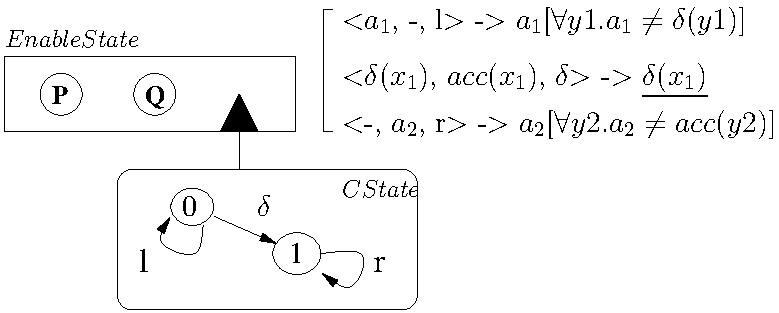
\includegraphics[width=\linewidth]{XFIG/Enable1}
  \\[1.3ex]
 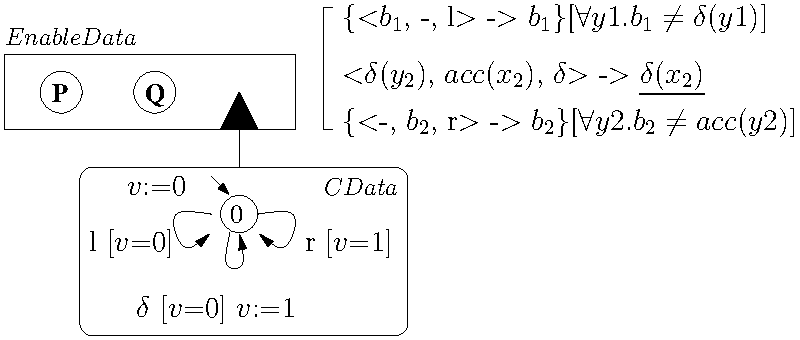
\includegraphics[width=\linewidth]{XFIG/Enable2}
  \caption{Two pNet encodings for  Enable }  \label{schema:enable-pnets}
\end{minipage}
  \hspace{2mm}
\begin{minipage}{6cm}
  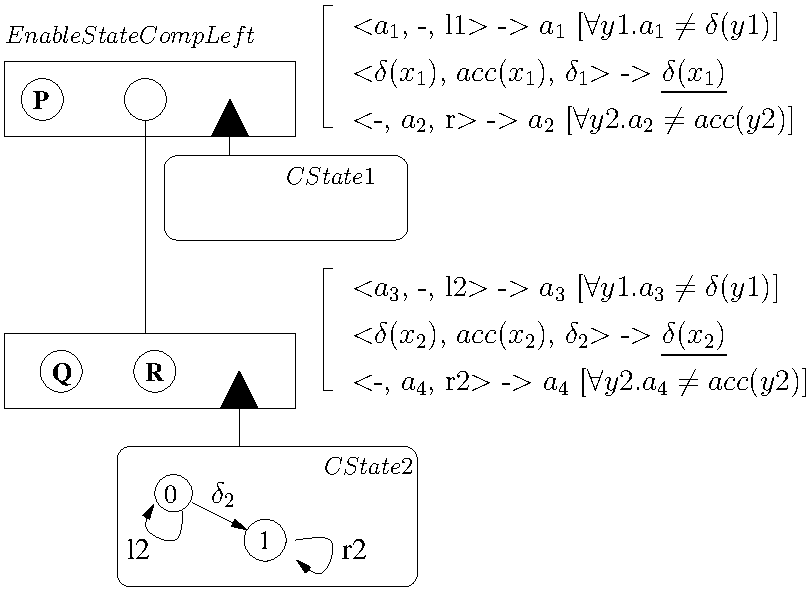
\includegraphics[width=\linewidth]{XFIG/P-QR}
  \caption{Composed pNet for ``P>>(Q>>R)''}  \label{schema:enable-composed}
\end{minipage}

\end{figure}

	To give simple intuitions of the open pNet model and its semantics, we use
	here a simple example based on the ``Enable'' operator of the LOTOS language.
	In Fig. \ref{schema:enable-pnets}, we show 2 possible encodings of the  
	``Enable'' operator.
	In the Enable expression ``P>>Q'', an \texttt{exit(x)} statement within P
	terminates the current process, carrying a value $x$ that
	is captured by the \texttt{accept(x)} statement of Q. 
	
	We use a simple action algebra,
	containing two constructors $\delta(x)$ and $acc(x)$, for any
	possible data type of the variable $x$, corresponding to the
	statements \texttt{exit(x)} and \texttt{accept(x)}. Both $\delta(x)$
	and $acc(x)$ actions are
	implicitly included in the sorts of all processes.
	We need no specific predicate over the action expressions, apart
	from equality of actions. 
	In the first encoding $Enable1$, in the upper part of
	Fig. \ref{schema:enable-pnets}, we use a controller $C_1$ with two
	states, and simple control actions $l, r, \delta$. The second encoding
	$Enable2$ uses a data-oriented style, with a single state controller, and a
	state-variable $s_0$, with values in $\{0,1\}$.

        In this example we use \emph{synchronised
          actions}, to express actions that cannot be further synchronised, like the
        $\tau$ silent action of CCS. We denote them as any action expression with the text
        underlined, as e.g. $\underline{\delta(x_2)}$. Such
        synchronised actions do not play any special role for defining
        the semantics of pNets, but as one can expect, will be crucial
        for defining weak equivalences.
	
	Note that synchronisation vectors are defined in a parameterised
	manner:  the first and third lines represent one vector
	for each parameterised action in the Sort of hole $P$
	(resp. $Q$). This notation can also use predicates, as in the first
	case, in which we want the vector to apply to any action of $P$
	except $\delta(z)$.
	
	In Fig. \ref{schema:enable-composed}, we enrich our example by
	composing 2 occurences of the Enable1 pNet. To simplify,
	we only have represented one instance of the synchronisation vector set,
	and of the controller.




\section{Operational Semantics for Open pNets}
\label{section:op-semantics}

The semantics of open pNets will be defined as an open automaton, that
is an automaton where each transition composes transitions 
of several
% \noteSB{These should all be pLTSs, right? Or did I miss
%  something?}\noteEM{Hum, nor really, something intermediate; the actions there can be
%  parameterised actions, but the label has no guard and no
%  assignments}
LTSs with the actions of some holes; the transition occurs if some predicates hold,
and can involve a set of state modifications. Each state of an open
automaton has a set of \emph{state variables} that can be assigned by
incoming transitions. Strictly speaking, the LTSs at the leaves of the
open automaton are a restricted form of pLTSs, where labels are
parametrised actions, but include no guard nor assignments.

\begin{definition}[Open transitions]
	\label{def:OpenTransitions}
	An \emph{open transition} $OT$ over
        % a set  $\langle S_i,s_{0 i}, \rightarrow_i\rangle^{i\in I}$ of LTSs,
        a set $J$ of holes, %with sorts $Sort_j^{j\in J}$
        and a set of states $\mathcal{S}$ is a structure of the form:	
	\begin{mathpar}
	\inferrule*[myfraction=\reddottedrule]
	{%\{s_i~{\xrightarrow{a_i}}_i ~s_i^{\prime}\}^{i\in I},
		\{\xrightarrow{\beta_j}_j\}^{j\in J}, \Pred\,, \Post}
	{s \xrightarrow {\alpha}s'}\,,
	\end{mathpar}
	where $s, s'\in\mathcal{S}$, the $a_i, \beta_j, \alpha$ are
        action expressions,
        % $s_i{\xrightarrow{a_i}}_i s_i^{\prime}$ is a transition of the 
	% LTS $\langle S_i,s_{0 i}, \rightarrow_i\rangle$
        $\beta_j$
        is an action of the hole $j$, and $\alpha$ is the resulting action
        of $OT$. \Pred\ is a predicate
	over the variables of the terms, labels, and states $s_i$,
        $\beta_j$, $s$, $\alpha$. \Post\ is a set of equations that  
	hold \emph{after the open transition}, represented as a
        substitution $\{x_k\gets e_k\}^{k\in K}$  
	where $x_k$ are variables of $s'$ and $s'_i$, whereas $e_k$ are
        expressions over the other variables of the open transition.
\end{definition}


\begin{definition}[Open automaton]
	\label{def:open-automaton}
	An \emph{open automaton} is a structure\\ $A =
	\langle J,\mathcal{S},s_0,\mathcal{T}\rangle$ where:
	\begin{itemize}
		\item[$\bullet$]  $I$ and $J$ are  sets of indices,
	%	\item[$\bullet$]  $LTS_i^{i\in I}$ is a family of LTSs,
		\item[$\bullet$]  $\mathcal{S}$ is a set of states and $s_0 \in \mathcal{S}$ the initial state,
		\item[$\bullet$] $\mathcal{T}$ is a set of open transitions and, for each
		$t\in \mathcal{T}$, there exist $I'$, $J'$ with $I'\subseteq I$, $J'
		\subseteq J$, such that $t$ is an open transition over $J'$,
		and  $\mathcal{S}$.
		
	\end{itemize}
\end{definition}
	

%
%Then the semantics of a pNet is characterized by a set of {\em open
%transitions}, where the hypotheses on process parameters are
%replaced by 1) transitions of the pLTSs at the leaves, and 2) formal
%hypotheses on the transitions of the holes. A {\em predicate} is used
%to relate the parameters and names appearing in the actions of the
%leaves and the holes involved in the rules, but also appearing in  the resulting action.

% \TODO{Relate to the algorithm, or even move to section 5}
The \emph{states} and the shape of \emph{predicates} in the
transitions
of an open automaton representing the semantics of a pNet
have the following specific structure.

\paragraph{States of open pNets.}\label{def-states}
  A state of an open pNet is a tuple of the
  states of its leaves (in which we denote tuples
  in structured states as $\triangleleft\ldots\triangleright$).
  For any pNet p, let $\overline{\mathit{Leaves}} = \mylangle S_i,{s_i}_0, \to_i\myrangle^{i \in L}$ be the set of pLTS at its leaves,
  then $\mathit{States}(p) = \{\ostate{s_i^{i\in L}}
  |\, \forall i\in L. s_i \in S_i\}$.
A pLTS being its own single leave:
  $\mathit{States}(\mylangle S,s_0, \to\myrangle) = \{\ostate{s}|\, s \in S\}$.
The initial state is defined as:
$\mathit{InitState}(p) = \ostate{{{s_i}_0}^{i\in L}}$.


%% \begin{example} \emph{State of a pNet}
%%   The states of pNet \texttt{EnableCompL} are:
%%   $\triangleleft 00 \triangleright, \triangleleft 10 \triangleright, \triangleleft 11 \triangleright$
%% \end{example}

\paragraph{Predicates.}
Let
$\mylangle\overline{\pNet},J,\symb{SV}_k^{k\in K} \myrangle$
be a pNet. Consider a synchronization vector $SV_k$, for $k\in K$. We build a
predicate $\MkPred$ relating
the actions of the involved sub-pNets and the resulting actions. This predicate verifies:
\begin{multline*}
  \MkPred(SV_k, a_i^{i\in I}, b_j^{j\in J}, v)\Longleftrightarrow
  %% \begin{array}{l}
  \exists {(a'_i)}^{i\in I},
          {(b'_j)}^{j\in J},v'.\\
          SV_k={(a'_i)}^{i\in I}, {(b'_j)}^{j\in J}\rightarrow v'
          \land
          \forall i\in I.\, a_i=a'_i\land \forall j \in J.\, b_j=b'_j \land v=v'
\end{multline*}

%% \end{array}


%% This definition is not constructive but it is easy to build the
%% predicate constructively by brute-force unification of the sub-pNets
%% actions with the corresponding vector actions, possibly followed by a simplification
%% step. 

\begin{example}[An open transition]\TODO{change for Enable example}
  Transition $OT_1$ of the pNet $EnableCompl$ is generated by
  combination of the first vector of its root node, with
  the second vector of its $2^{nd}$ node. Its generated predicate is
  trivialy true. The global states shows that controler $C_3$ has
    changed from state 0 to 1.

    \TODO{add another example to illustrate assignements/Post}

  \label{OT:example-1}
        \begin{mathpar}
	  OT_1  =
          \inferrule*[myfraction=\reddottedrule]
	{\{\xrightarrow{\delta(x3)}_P ~~
          \xrightarrow{acc(x3)}_Q \} ~~
          [\forall z. acc(x3) \neq \delta(z)]
        }
	{\ostate{0,0} \xrightarrow {\underline{\delta(x3)}} \ostate{1,0}}
	\end{mathpar}
\end{example}


\paragraph{Structural Semantic Rules:}
The semantics of pNet in term of open automata has been defined in
\cite{henrio:Forte2016}, in the form of 2 structural rules, one for
pLTSs, one for pNet nodes. These rules are slightly improved, adding guards in the synchronisation vectors and syntax for universal quantifier in the guards (see~\cite{Avocs-RR}).
  
In \cite{henrio:Forte2016} we also proved:
\begin{theorem}[Finiteness]
  \label{Th:finiteness}
  Given an open pNet $pnet=\mylangle \overline{\pNet},\overline{S}, \symb{SV}_k^{k\in K}\myrangle$ with leaves $l_i^{i\in I}$ and holes $h_j^{j\in
  J}$, if the sets $I$ and $J$ are finite, if the synchronisation vectors of all pNets 
  included in  $pnet$   are finite, and if
$\forall i \in L.\, finite{(states(l_i))} \text{ and } l_i$
has a finite number of state variables, then its semantics is an open automaton 
$\mathcal{T}$ with finitely many states and transitions.
\end{theorem}
  Remark that all the elements of such pNets and open automata being
symbolic, they can represent many classes of unbounded systems. 

\begin{proof}
  \TODO{I tentatively copied the proof here, from RR-8898.
the proof of the finiteness theorem refers to SOS rules Tr1 and
  Tr2. So maybe we must include (and explain) these here. One problem
  is that these rules have been modified/improved with each new
  publication of pNets papers, so we have to decide which version we
  use here
    Then we should
    check if it is sufficient with this version of the algorithm, or
    if it can be make more precise (some added analysis of the
    behavior of matching/combining/filetring ?)}
  The possible set of states of the open-automaton is the cartesian
  product of the states of its leaves $pLTS_i^{i\in L}$, that is finite by
  hypothesis. So the top-level residual loop of Algorithm 1 terminates provided each 
  iteration terminates. The enumeration of open-transitions in step 2b is bounded by the
  number of applications of rules Tr2 on the structure of the
  pNet tree, with a finite number of synchronisation vectors applying
  at each node the number of global open transition is finite. Similarily rule Tr1 is 
  applied finitely if the number
  of transitions of each pLTS is finite. So we get finitely many deduction trees, and
  open-transitions which ensures that each internal loop of Algorithm 1 terminates.
  \end{proof}

\section{Generation of Open Automata}
\label{section:implementation}
In this section we describe the algorithm implementing the pNet
semantics, the interaction with the Z3 SMT solver, and we show the
result on our example. Under the hypotheses of Theorem \ref{Th:finiteness}
this algorithm terminates. 

%% \noteSB{
%% line 11: Would it not be better to prune unsatisfiable transitions
%% on-the-fly, \ie inside the loop?}
%% \noteEM{Not so easy, it would require a proof... on one side this
%%   would implement reachability on the fly; but there is the question
%%   of collecting the assignments of the state variables, that are used
%%   in the sat check !}

\begin{algorithm}[h]
  \caption{Open Automaton Generation}
  \label{alg1}
\begin{algorithmic}[1]
\Require A pNet $P$ (can be a pLTS, but not a hole)
        %\qquad \hl{\textbackslash\textbackslash~SB: was `` pn ''}
\State Initialize sets $U=\{\mathit{InitState}(P)\}$ and $E=\emptyset$,
for unexplored and explored global states, respectively; $L=\emptyset$ for the resulting OTs;
\While{!$\mathit{isEmpty}(U)$}
	\State Choose $S$ in $U$; remove $S$ from $U$, add $S$ to $E$;
        %\qquad \hl{\textbackslash\textbackslash~SB: was `` Choose $S$ in $U$ ''}
	\State $\mathit{OTs} = \mathit{MakeTransitions}(P, S)$;
	\For {each $\mathit{OT} \in \mathit{OTs}$}
          \State Add $\mathit{OT}$ to $L$;
          \State Let $S'$ be the target state of $\mathit{OT}$
          Add $S'$ to the unexplored states if necessary:
	  \IfThen{($S' \not\in U \cup E$)}{Add $S'$ into $U$;}
	  \EndFor
\EndWhile
\State \ERIC{Prune the unsatisfiable open transitions in $L$ using the SMT
solver; only keep reachable global states;}
\State \Return $\mathit{OA}=(\mathit{InitState}(P),L)$;

\end{algorithmic}  
\end{algorithm}

Algorithm~\ref{alg1} starts with an open pNet, and builds its set of open
transitions. Its main loop is a classical residual algorithm: starting
from the initial global state, it picks a state in an unexplored set, and
computes all possible OTs, adding their target states in the
unexplored set, until this set is empty.

\ERIC{Before the SAT checking step, it may contain symbolic transitions that
do not have valid ground instanciations. This is not logicaly
incorrect, but is naturaly not an optimal representation. So we prune
these UNSAT transitions: at the root of the pNet, the predicate of each OT is translated
into SMTlib assertions, and checked for satisfiability.
The final open automaton includes all satisfiable OTs, and the set of
reachable global states.}
%By construction, due to the
%satisfiability test in line 6, it only produces the set of states reachable
%through a sequence of satisfiable open transitions.


The inside loop (\emph{MakeTransitions} method) applies recursively
the semantic rules following the structure of the pNet.
When applied to a pLTSs at the leaves, we simply take the pLTS transitions of the
corresponding local state and use the semantic rule to build the OT\footnote{%
%
  We omit detailed presentation of this case for the sake of brevity.
%
}.
When applied to a pNet node we use two methods, combining and
matching, to generate the open transitions in a hierarchical manner,
as shown in Alg.~\ref{alg2}. This method directly manages the
holes of the node, so \emph{MakeTransitions} is never called on a hole.


%
%% \noteInSB{Algorithm~\ref{alg2}, as presented below is not
%%   well-defined: when we reach the leaves, a pLTS does not have any
%%   subnets, hence the loop in lines 2--4 is empty and so is the list
%%   $l$. $\mathit{Combining}(l)$ is then called on an empty list...}

%\noteInSB{Line 2: Tr1 and Tr2 are the semantic rules, right?}

%% \noteInSB{Line 6: Nothing in the assignment $\overline{comb} =
%%   \mathit{Combining}(l)$ depends on $sv$.  Hence, this should probably
%%   be done outside of the loop.}

%% \noteSB{Line 7: There are two type mismatches here: $ot$ is an open
%%   transition, whereas $\mathit{Matching}$ is a predicate\mdash one
%%   cannot assign a predicate to an open transition.  Furthermore, in
%%   the definition of $\mathit{Matching}$, below, $C_n$ is an open
%%   transition, whereas $\overline{comb}$ is a {\em set} of open
%%   transitions, so this call does not type either. There is probably
%%   another inner loop over all tuples of OTs in $\overline{comb}$; even
%%   so the open transition has to be defined completely, not just the
%%   predicate\mdash what is the value of $Post$ for the new transition?
%%   Maybe $\mathit{Matching}$ should not be a predicate, but an OT?
%%   Finally, how is $\mathit{hole}$? (I have removed $v$\mdash here and
%%   in the parameters of the definition of the $\mathit{Matching}$
%%   predicate, because the text in the paragraph ``Matching'' says that
%%   $v$ is fresh.)}
%% \noteEM{Done, please check the new version}

%\noteInSB{Line 8: When is $\mathit{Filter}(ot)$ called?}

\begin{algorithm}[h]
\caption{MakeTransitions() \em{for a pNet node}}
  \label{alg2}
\begin{algorithmic}[1]
\Require a pNet node $P$ with subnets $\overline{sn}$ and holes $\overline{hole}$; a global state $S$.
\State Initialize empty list $l$ and set $L$ for sub-transitions and transitions, respectively;
	\For{each $\mathit{Subnet}$ in $\overline{sn}$}
        \hfill $\setminus \setminus$ Recursively apply the semantic rules on the subnets
           \State Store $\mathit{MakeTransitions}(Subnet, S)$ in $l$;
	\EndFor
	\State $\overline{comb} = \mathit{Combining}(l)$;
	\For{ each $sv \in SV$ and each $comb \in \overline{comb}$ }
           \State $ot = \mathit{Matching}(sv, \overline{\mathit{comb}}, \overline{\mathit{hole}})$;
           \IfThen{($ot$ is defined)}{Store $ot$ in $L$; ~~~ $\setminus \setminus$ if $\mathit{Matching}()$ succeeds}
	\EndFor
\State \Return $L$;
\end{algorithmic}  
\end{algorithm}



%
%For holes, their behaviour is unspecified, it doesn't have an exact
%external presentation of action. We only give an action variable to each hole
%and treat it as hole behaviour to suppose working status of the
%hole.
%% Here should have a constraint that this variable belongs to the sort of hole.
%In every case, the hole behaviours are unchanged, so we
%only make the combinations of subnets' open transitions. 
%


\def\inactive{\{-\}}
\paragraph{Combining.}
The combining method enumerates all the possible behaviours of the
subnets as all the possible combinations of their open transitions.
Assume that there is a collection of $n$ subnets.
%% \noteSB{These variables are not used and conflict with the returned
%%   set $L$ in Alg.~\ref{alg2}, on one hand, and control states $s_i$ of
%%   the subnets, on the other.}
%% \st{$L = {s_1, s_2, ...,  s_n}$;}
We denote $\overline{ot}_i$ the set of open
transitions of the $i$-th
subnet (obtained in line~3 of the algorithm); %% $s_i$ and 
``$-$'' means that the subnet is not involved.
The combination $\overline{comb}$, a set of n-tuples, is the
cartesian product:  
$\overline{comb} = (\inactive\cup \overline{ot}_1) \times (\inactive\cup \overline{ot}_2)\times \dots \times (\inactive\cup \overline{ot}_n)$.

%Algorithm 2 shows the combining algorithm for enumerating all possible
%working status combinations from subnets. Dealing with a list $TR$
%containing  sets of open transitions from different subnets,
%the algorithm choses one of sets $L_{ot}$ and does combining on the
%remaining part of $TR$ recursively. The case when a subnet is not working is
%managed by adding a $null$ into the $L_{ot}$.



\paragraph{Matching.}
The \emph{Matching} method builds the OTs of a pNet node from those of
its subnets.
For each synchronisation vector and each possible
combination of behaviours of the subnets, as generated by the \emph
{Combining} method, it builds the corresponding open transition.
Here, we only detail the construction of the predicate.
From a synchronization vector
$sv = \left((a'_i)^{i\in I} (b'_j)^{j\in J}\rightarrow v'\right) \in SV$
and its guard $G_k$; a tuple of open transitions
$C = ({ot}_i)^{i \in [1,n]} \in \overline{comb}$, such that, for each $i \in [1,n]$, either $ot_i = -$, or the result action of $ot_i$ is $a_i$; the hole behaviours $\mathit{Hole} = (b_j)^{j \in J}$; and a fresh variable $v$, representing the result action of the OT under construction, we build the predicate:
%
\begin{multline*}
  \mathit{MkPred}(sv, C, \overline{\mathit{hole}}) = 
  \\
  (\forall i\in I, a_i=a'_i) \land
%  (\forall i \not\in I, ot_i = -) \land
  (\forall j\in J, b_j=b'_j) \land
  (v=v') \land G_k.
\end{multline*}


\paragraph{Filtering.}
While matching a vector with a combination tuple, \emph{Matching}
tries to filter out some incompatibilities; there may be several
reasons why the matching would fail: 
\begin{itemize}
  \item if some subnet is marked as inactive in the vector, and the
    chosen combination has an active behaviour at this position,
  \item if some subnet action expression in the vector does not match (by
    pattern-matching) the corresponding action expression in $C$,
  \item or if the whole set of active subnet actions in the vector
    cannot be matched (by unification) with the corresponding action expressions
      on the tuple $C$.
\end {itemize}

%\st{Each of these possible filters is more precise than the previous
%  ones. But e}
Even when unification succeeds, it is still possible that
the resulting predicate would be unsatisfiable, because of some
incompatibility involving the guards. In our algorithm, we choose to
apply only the simplest filter inside the \emph{Matching} method
(before applying the predicate and OT construction). Matching and
unification  will be checked later, together with the guards collected
from synchronisation vectors and from pLTS transtions, using the
satisfiability check in the SMT engine.


\subsection{Management of state variable assignments}


In a pLTS, there may be several incoming transitions 
that assign potentially different values to a state variable.
To handle such cases, the algorithm manages, for each pLTS state, a
list of expressions collected from the assignments of each state
variable. %% $v$.
%% The list we used contains triples <$v$, $S$, $AssignRH$> 
%% where $v$ is the variable in pLTS, $S$ is its owner state and
%% $AssignRH$ is a list of expressions over other variables in the right
%% hand side of assignments of $v$.
% As a pragmatic extension to the formal definition, we also manage
% ``global variables'', defined in all states of the pLTS.
For a global state in the open automaton, the set of state
variables (which may be used in a transition) %% will simply be
is the disjoint union
of sets of state variables of the individual pLTS states constituting this
global state.
%There are some assignment on the variables in each of states of the pLTS (state variables), or just as global states of it (global variables). There is usually not only one assignment for a state variable, miss of them may drop the unsatisfiable results. In order to avoid such mistakes, 
\TODO{these assignment sets collect potential assignments from all OTs
  in the generated automaton. If we minimize the generated state
  space, we will get less assignements, and potentialy also get better
  minimization... }

%% \QIN{
%% The list we used contains several triples <$v$, $S$, $AssignRH$> to
%% record the information of both state and global variables of the pLTS,
%% where $v$ is the variable in pLTS, $S$ is its owner state and
%% $AssignRH$ is a list of expressions over other variables in the right
%% hand side of assignments of $v$. It means the variable is global in
%% the pLTS belonging to all the states, if $S$ is $null$. We update the
%% list of record triples every time Tr1 is applied. Then we can track
%% all the possible (symbolic) value of the variables when computing open transitions.
%% }

\subsection{Pruning the unsatisfiable results}
\label{section:pruning}

\begin{figure}[t]
\begin{mathpar}
    ot = \openrule{\{s0 \xrightarrow{fail(true)} s0, t0 \xrightarrow{resume(false)} t0\}, ~~\{\xrightarrow{hb}\},~~fail(true)=fail(b_1)\\
    \OTland resume(false)=start(b_2)\OTland hb=fail(b_0)\OTland v=\underline{fail}\OTland b_1=b_2\\
    \OTland (b_1\lor b_2) \Rightarrow b_0, ~~\{\}}
    	   {\ostate{s0,t0} \xrightarrow{v} \ostate{s0,t0}}
  \end{mathpar}
\caption{One of the unsatisfiable open transitions \TODO{to be changed}}  \label{schema:unsat-ot}
\end{figure}

Our matching/filtering strategy builds some transitions where
the predicates express incompatible constraints. Even if having an
unsatisfiable (symbolic) transition would not be incorrect,
we choose to minimize the open automaton (\ie its number of
transitions and states), by checking the predicates for satisfiability.
In Fig.~\ref{schema:unsat-ot}, we show an 
unsatisfiable open transition 
from the open automaton of our running example. It shows the case where
the failure controller performs a ``$\PortFail$'' action, while the timer
executes a ``$\PortResume$''. The chosen synchronization
vector (SV0 from Fig.~\ref{schema:ArchFailure:pNet}) does not match
with these actions, since it expects $\NameTimer.\PortStart$. This
  mismatch is materialised by the predicate
fragment ``$\mathit{resume}(\false)=\mathit{start}(b_2)$''. 

Checking satisfiability requires some symbolic computation
on the action expressions and the predicates, which
may depend on the specific theory of the action algebra datatypes. 
The ``Modulo Theory'' part of SMT solvers is important here, so that
the solver can use specific properties of each action algebra.

\subsection{Computing reachable state space on the fly}
\TODO{add a high level description of the new strategy, discuss
  decidability/approximation of the SAT checking, express some
  ``minimality'' property}

The basic algorithm from the previous section potentialy explores some
areas of the global state-space that will not be reachable after
checking the OTs' predicates for satisfiability. Incorporating the
satisfiability check inside the residual algorithm will definitely
save some of these useless computation. More precisely, it will still
create, and submit to Z3, the OTs at the ``border'' of the state-space, but
not the transitions issued from non-reachable global states.

\ERIC{But there is more to this. As mentionned above, we collect all
possible (symbolic) assignments of state variables, in the
computed open automaton. By avoiding building the OTs coming from
unreachable states, we also avoid adding the corresponding assignments
to the variables of their target states. The set of possible
assignments is an over approximation of possible values of the
variables of such state, so narrowing it means we get a better
approximation, and potentialy more informations, that can be used to
the SAT check of subsequent transitions.}
\TODO{Beware, I think this is dangerous... Xudong, do we really use
  assignment information in SAT checking ? In the ``smart'' version, I
  think we must NOT use it, because we do not yet have collected all
  possible assignments.}

Algorithm~\ref{alg3} implement this new stategy: \TODO{Explain
  significant detials}

\begin{algorithm}[h]
  \caption{``Smart'' Reachable Open Automaton Generation}
  \label{alg3}
\begin{algorithmic}[1]
\Require A pNet $P$ (cannot be a hole)
        %\qquad \hl{\textbackslash\textbackslash~SB: was `` pn ''}
\State Initialize sets $U=\{\mathit{InitState}(P)\}$ and $E=\emptyset$,
for unexplored and explored global states, respectively; $L=\emptyset$ for the resulting OTs;
\While{!$\mathit{isEmpty}(U)$}
	\State Choose $S$ in $U$; remove $S$ from $U$, add $S$ to $E$;
        %\qquad \hl{\textbackslash\textbackslash~SB: was `` Choose $S$ in $U$ ''}
	\State $\mathit{OTs} = \mathit{MakeTransitions}(P, S)$;
%%        \State Store $\mathit{OT}$ in $L$; 
	\For {each $\mathit{OT} \in \mathit{OTs}$}
        Check satisfiability of $\mathit{OT}$ using the SMT solver;
        \IfThen {$SAT(\mathit{OT})$}
                {\State \{Add $\mathit{OT}$ to $L$;
                  \State Let $S'$ be the target global state of $\mathit{OT}$
	          \IfThen{($S' \not\in U \cup E$)}{Add $S'$ into $U$;}
                  \}}
	\EndFor
\EndWhile
%%\State Prune the unsatisfiable open transitions in $L$ using the SMT solver;
\State \Return $\mathit{OA}=(\mathit{InitState}(P),L)$;

\end{algorithmic}  
\end{algorithm}

\TODO{Candidate theorems:
  - All reachable states from algorithm 1 are kept by Algorithm 3\\
  - Algorithm 3 computes an open automaton that is minimal with
  respect of SAT checking decidability.\\
  I have problem with minimality... Because of the ``two phases'' SAT
  checking that we have now, because we cannot use incomplete sets of
  variable assignments during the ``smart'' phase, and use them later,
minimality becoomes trivialy equivalent in the original and smart algorithms...}


\subsection{Translation to SMTlib}

We check the satisfiability of each open transitions
using the SMT solver Z3.
%More precisely, we translate
%the OT predicate into an SMTlib assertion in the context provided by
%the possible state variable assignments in the source state.
In this
section, we describe the translation of the algebra presentation, of
assignments, and of the predicates.

Our implementation submits satisfiability requests to
Z3 using its JAVA API. Here, for readability, we
show the Z3 code using its SMT-LIB input language.
Note that in the previous sections, the OTs were displayed in a
  simplified, human readable form. The input and output of our tool, and
  also the generated SMTlib fragments, are
  slightly more difficult to read, in 
particular because of structured names for the fresh variables generated
by the algorithm, allowing tracability of the result~\cite{Avocs-RR}.

Figure~\ref{schema:smt-lib} shows the translation of the
transition of Fig.~\ref{schema:unsat-ot}
in the SMTlib syntax.
It contains the declaration
of the BIP action algebra sorts 
and constructors, then the declaration of variables, and finally the
predicate to be checked, encoded as a set of assertions.
Here the behavior of the hole ``B'' appears as a variable
``|hb\_B:13:1|'', and line 10 shows the constraint that matching with
a synchronisation vector has imposed on the behavior of ``B''.
Here we display also the diagnosis (``sat'' or ``unsat'') generated by Z3.

\begin{figure}[t]
  %  \centerline{\includegraphics[width=12cm]{XFIG/SMTLIB2}}
    \centerline{\includegraphics[width=\linewidth]{XFIG/SMTLIB3}}
  \caption{The input of the Z3 solver in SMT-LIB language and the output result\TODO{Change}}  \label{schema:smt-lib}
\end{figure}

By lack of space, we have only shown here a use-case with boolean data
parameters, so we only require the basic SAT capability of the Z3
engine. It should be clear that more involved examples will require
reasonning on predicates of various data types. Z3 provides theories for reasonning
on integers, bitstrings, enumerated types, arrays, etc.
We also need to deal with some universal quantification on free
variables occuring in the guards of synch vectors.
For other data structures usual in such models, like records, or
recursive structures, the user will have to develop its own theories.
Decidability of these theories will condition the completeness of the
satisfiability check, and the decidability of model-checking or
bisimulation checking.




%% \begin{figure}[t]
%%   \centerline{\includegraphics[width=10cm]{XFIG/Interaction}}
%%   \caption{The architecture of the interaction between pNet API and Z3}  \label{schema:interaction}
%% \end{figure}

\paragraph{Production of the SMT-lib code}
  To build the input submitted to Z3 for each OT,
we translate the algebra presentation, the predicates and the
variable assignments into Z3 (Java-API) calls.
% The $presentation$ and the predicates are translated separately. 

\emph{Translation of action algebra presentation.}
In~\cite{Avocs-RR}, we  define the translation of an algebra presentation into
SMTlib declarations (\texttt{declare-datatypes} and
\texttt{declare-fun}). We also formalize a condition of well-formedness of pNets ensures that the generated code is correct,
and will not raise runtime errors in the SMT engine. Note that the
\texttt{declare-datatypes} command comprises both the action
constructors from table \ref{table:BIPalgebra} and also the constant action
names from our example.
Additionally, we will include axiomatisation of any required functions
and predicates of the presentation data-types.


%% \paragraph{Translating assignments into predicate terms.}
%% State variable assignments that were collected during the open
%% automaton are used when generating the SMTlib asserts (see
%% App.~\ref{appendix:translating-assignments}). \noteSB{I am not an expert of Z3 or SMT-LIB, but the clause '\texttt{(= t (- t 1))}' looks very suspicious to me.}\hl{This appears in
%% line 10 of Fig.~\ref{schema:smt-lib}, which encodes possible values of
%% the variable $t$ of the timer.}

%The assignments are also taken into account when checking the
%satisfiability of the open transitions as they represent the value of
%the variables involved in an OT. In order to do that, we employs a
%translation from assignments into term of predicates. The assignments
%required to be translated are only those belong to the variables
%contain in the start states of the open transitions. The assignments
%are represented as equations between the variables and the expressions
%on the right side of assignment. For the assignments of the same
%variable, we do not figure out which state is the precursor of current
%state, we keep all these possible equations instead, and generate the
%disjunction of these equations. The state could always move to the
%target state if there exists one of the values of its variable
%satisfies the guard.
%%\TODO{It won't matter the variable of the next state
%%except that the right hand side expression contain its variables. This
%%is a problem left to be solved in our future work. WHICH PROBLEM ?}
%After that, for the assignments of the different variables, we generate a conjunction of them. This way we obtain a new term of the predicate involving assignments of the variables.

%% State-variable assignments are also treated as a part of the
%% predicates when checking the satisfiability. % Here we need conduct some
%% % translations,
%% For each assignement in a $\Post$ predicate, such as $\{s_0 \leftarrow 1\}$ in section
%% ~\ref{section:op-semantics}, we translate it into an equation
%% $s_0=1$. For several assignments of the same variable in the same state,
%% we generate the disjunction of 
%% these equations. Correspondingly, we generate a conjunction for the
%% assignments from different variables. 


\emph{Translation of open transitions.}
In~\cite{Avocs-RR} we formally define all steps of the translation of each
open transition, including:
%
\begin{itemize}
\item collect all variables in the transition, and declare them (using \texttt{declare-const})
\item check well-formedness and correct typing of expressions,
\item translate the predicate into a conjunction of assertions,
\item if present in the source state, translate the state-variable
  assignments into a disjunctive assertion.
\end{itemize}
%
This translation ensures that no runtime error will occur
in the SMT engine.

Figure~\ref{schema:smt-lib} shows the decomposition of the
predicate into a set of asserts, each encoding an elementary equality,
inequality, or a guard. 
The result (sat or unsat) of the final \texttt{check-sat} command in
the translation () is then decoded.

\section{Use-cases}
\TODO{new section here, showing various features on different examples}

\subsection{Enable operator} in Lotos, with (equivalent) state-based and data-based encodings; Associativity of Enable;

\subsection{simple communication protocol} specification and implementation;

\subsection{BIP FailureTimer architecture}


\label{section:FailureTimerMax}
\label{section:BIParchitectures}
\label{section:examples}

\TODO{use a simpler running example (e.g. Lotos Enable operator ?), and move the BIP example to a dedicated section at the end}

As a running example we use the Failure Monitor architecture from the
CubETH nanosatellite on-board software
case-study~\cite{CubETH-case-study} realised using BIP.
The architecture-based design process in BIP takes as input a set of
components providing basic functionality of the system and a set of
temporal properties that must be enforced in the final system.  For
each property, a corresponding architecture is identified
%\,\footnote{%
%
%  The current approach relies on taxonomies of predefined
%  architectures.  Future work may include automatic synthesis of
%  architectures from, \eg CTL~\cite{BaierKatoen2008} formulae.
%
  %}
  and applied to the model, thereby potentially introducing additional
coordinator components and modifying the connectors that define
synchronisation patterns among ports of components.

\begin{figure}[t]
  \centering
  \includegraphics[width=0.8\columnwidth]{XFIG/BIPspec-ArchFailureTimerMax-v2}
  \caption{The BIP specification of the Failure Monitor architecture}
  \label{schema:ArchFailure:BIP}
\end{figure}

Figure~\ref{schema:ArchFailure:BIP} shows a refined version of the
Failure Monitor architecture used in~\cite{CubETH-case-study}.
Contrary to standard BIP models, architectures comprise one or several
\emph{operand} components, whereof only the set of \emph{ports} is
given.  Here, the operand component is $\NameOprnd$ and its interface
consists of the ports $\PortFinish$, $\PortResume$ and $\PortFail$.
The two \emph{coordinator} components\mdash $\NameCtrl$ and
$\NameTimer$\mdash are standard BIP components insofar as they also
have their \emph{behaviour} specified by finite automata extended with
local data variables.  Transitions of these automata are labelled with
the ports of the corresponding components, Boolean guards and update
functions on local variables.  For instance the loop transition
$\tstate{1} \goesto{\PortTick, \GuardTick[], \TimerUpd[]} \tstate{1}$
in the $\NameTimer$ component is labeled by the port $\PortTick$, it
can be fired only when the current value of the local variable $t$ is
greater than $0$.  Upon firing, this transition decrements the value
of $t$ by $1$.  When omitted, the default guard (\resp update
function) is the constant predicate $\true$ (\resp the $\mathit{skip}$
operator).  The constant $\mathrm{Max}$, in $\tstate{0}
\goesto{\PortStart, \TimerInit[]} \tstate{1}$, is a parameter of the
architecture.

Connectors are hierarchical, tree-like structures with component ports
at the leaves.  They define sets of \emph{interactions}, based on the
attributes of the connected ports~\cite{BliSif08-acp-tc}, which may be
either \emph{trigger} (triangles in Fig.~\ref{schema:ArchFailure:BIP})
or \emph{synchron} (bullets in Fig.~\ref{schema:ArchFailure:BIP}).
%
If all sub-connectors of a connector are synchrons, then an
interaction may be executed by the connector only if each subconnector
can contribute.
%
If at least one of the sub-connectors is a trigger, then any
interaction consisting of contributions of any set of sub-connectors,
\emph{involving at least one of the triggers}, can be executed.
%
For instance, the two ports $\NameTimer.\PortStart$ and
$\NameCtrl.\PortFail$ are always synchronised, since they belong to
the same binary sub-connector, where they are both synchrons.  In
particular, this means that whenever the transition $\cstate{0}
\goesto{\PortFail} \cstate{1}$ is fired, so is the transition
$\tstate{0} \goesto{\PortStart, \TimerInit[]} \tstate{1}$,
initialising the timer.  The binary connector $\NameTimer.\PortStart
\bullet\!\!\!-\!\!\!-\!\!\!\bullet \NameCtrl.\PortFail$ is a
sub-connector of a hierarchical connector, where the port
$\NameOprnd.\PortFail$ is a trigger.  Thus, the above interaction can
only happen together with $\NameOprnd.\PortFail$, forming a
ternary interaction.  On the contrary, being a trigger, the port
$\NameOprnd.\PortFail$ can fire alone, forming a singleton
interaction.  The composition semantics of BIP systems consists in
firing exactly one interaction, enabled through at least one of the
top-level connectors, at each execution round.

Finally, \emph{priorities}\mdash defined by a strict partial order on
the set of possible interactions\mdash narrow the choice among the
enabled interactions at any given round.  The default priority is the
so-called \emph{maximal progress}, whereby among any two interactions
$a \subset b$ (as sets of ports), $b$ has higher priority than $a$.
For example, the port $\NameOprnd.\PortFail$ will never fire alone in
a global state, where both $\NameTimer.\PortStart$ and
$\NameCtrl.\PortFail$ are enabled.
%
%% Adding priorities $\NameOprnd.\PortFinish < \NameCtrl.\PortReset$ and
%% $\NameOprnd.\PortFinish < \NameOprnd.\PortResume$, ensures that, after
%% a failure, the operation performed by $\NameOprnd$ cannot finish
%% unless it is explicitly resumed or the system is reset.


Application of the Failure Monitor architecture ensures that, whenever
a failure is registered in the operand component, the system will be
reset, unless a resumption is registered within $\mathrm{Max}$ time
units (more details in Sect.~\ref{section:resultOA}).

\begin{figure}[t]
  \centering
  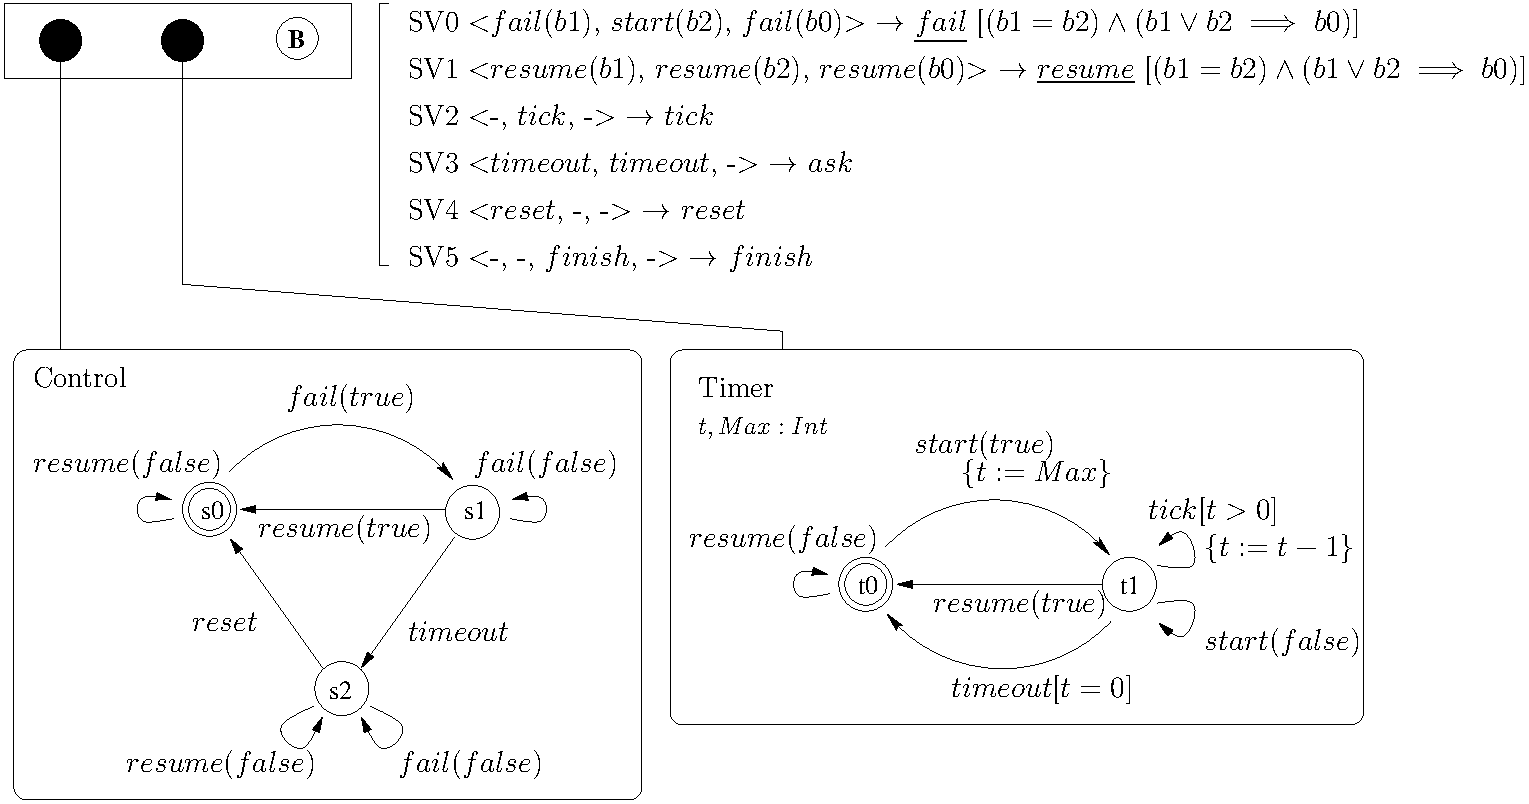
\includegraphics[width=0.9\columnwidth]{XFIG/FailureTimerPNET}
  \caption{pNet encoding of the Failure Monitor architecture}
  \label{schema:ArchFailure:pNet}
\end{figure}

Figure~\ref{schema:ArchFailure:pNet} shows a pNet encoding of the
above Failure Monitor architecture.  This encoding is structural: each
coordinator component is encoded as a pLTS, the operand
component\mdash as a hole; connectors of the BIP model are encoded as
synchronisation vectors.  Each connector that does not involve
triggers is trivially encoded by a synchronisation vector comprising
the same ports.  In order to encode the semantics of the connectors
involving triggers, we 1)~in the pLTS encoding the coordinator
components, add loop transitions to ensure that all ports involved in
such connectors are enabled in all states, 2)~associate a Boolean
value to each of these ports: the original transitions carry the value
$\true$ (\eg $\cstate{0} \goesto{\PortFail(\true)} \cstate{1}$), the
added loops carry the value $\false$ (\eg $\cstate{2}
\goesto{\PortFail(\false)} \cstate{2}$), 3)~add to the corresponding
synchronisation vectors the Boolean predicate encoding the connector
structure.  For example, $SV0$ encodes the connector discussed above:
the predicate $(b1=b2) \land (b1\lor b2 \Rightarrow b0)$ means that the
``true'' transitions $\NameCtrl.\PortFail$ and $\NameTimer.\PortStart$
can only fire together ($b1 = b2$) and whenever one of them fires,
$\NameOprnd.\PortFail$ must fire also ($b1 \lor b2 \Rightarrow b0$).
This encoding can be systematically obtained for any hierarchical BIP
connector~\cite{BliSif10-causal-fmsd}.
%
Although, for the sake of brevity, we omit priorities from the
encoding, this can be easily achieved, by introducing additional
Boolean variables for relevant ports~\cite{BarBliu15-offer-scico}.



\paragraph{Variations on the FailureTimer example}


\TODO{This is the original example from the Avocs paper, connectors slightly adapted so that it can be composed. Then Max Progress may be required to ensure properties}

For this example, the tool builds 184 open transitions, whereof 173
are detected unsatisfiable by Z3.  The resulting open automaton, with
3 reachable global states (out of the possible 6) and 11 open
transitions, is shown in Fig.~\ref{schema:resultOA}.

\begin{figure}[t]
  \centerline{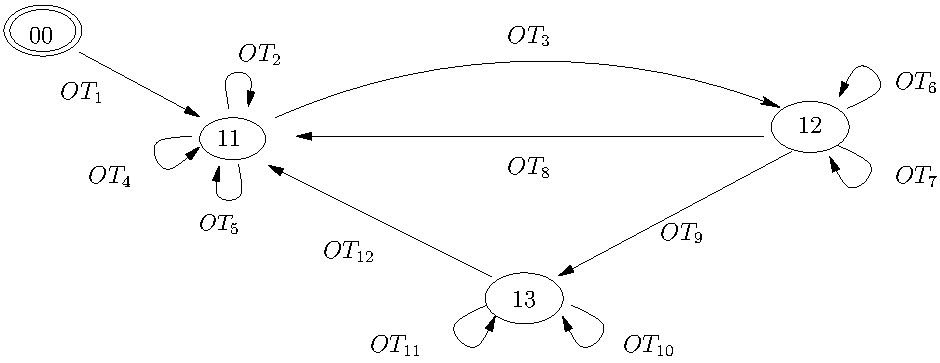
\includegraphics[width=12cm]{XFIG/FailureTimerOA}}
  \caption{Open Automaton for the Failure Monitor architecture}
  \label{schema:resultOA}
\end{figure}

To improve the readability of this figure, we used the following conventions:
we omit the transitions of the two pLTS, and the set of ``working''
holes; and we directly write the resulting action as first element of
each OT, rather than including it as an equality inside the
predicate.
%
%Notice, however that the loop transitions
%$\underline{\mathit{resume}}$ in states $\ostate{s0,t0}$ and
%$\ostate{s2,t0}$, corresponding, respectively, to open transitions
%$ot_2$ and $ot_9$ in Fig.~\ref{schema:ots} of
%App.~\ref{appendix:fullOutput}, involve $\OTvar{resume(false)}$ from
%the two pLTS, \ie only the hole, corresponding to the operand
%component of the Failure Monitor architecture, executes $\PortResume$.

Failure Monitor enforces 1)~the safety property \emph{``the
  system reset never happens, unless asked for by a timeout
  following a failure''}, formalised in CTL by
%
\[
\varphi \land \mathtt{AG} (\PortReset \rightarrow \varphi),
\quad\text{where}\
%
\varphi = \mathtt{A} [\lnot \PortReset\ \mathtt{W}\ \PortAsk]
\land \mathtt{A} [\lnot \PortAsk\ \mathtt{W}\ \PortFail],
\]
%
($\mathtt{W}$ being the \emph{weak until} operator) and 2)~the
liveness property \emph{``a reset will be fired when asked for by
  a timeout''}:
%
$\mathtt{AG}(\PortAsk \rightarrow \mathtt{AF}\ \PortReset)$.
%
The satisfaction of the safety property could be established by
applying symbolic model checking techniques.  However, in this
example, it is obvious by inspection of the open automaton.  The
satisfaction of the liveness property relies on the above observation
that in the state $\ostate{s2,t0}$ only the reset transition involves
$\NameCtrl$.  Therefore, under resonable scheduling assumptions,
$\PortReset$ will always be fired.


The safety
property \emph{``There is always a possibility to reset the system
  after a single failure''} (\ie without
  additional failures having to occur in the meantime) enforced by the
  Failure Monitor architecture can be specified using CTL as
    $\AG
\bigl(\PortFail \rightarrow \EX \EU[]{\lnot \PortFail}{
  \PortReset}\bigr)$.  Additional properties are provided in \ref{TimerRR}.

%% \TODO{it would be good to express here maybe 2 properties of the
%%   architecture, maybe one taken from the original study, and another
%%   one involving the timer data (number of ticks ?)}

\subsection{Composing 2 FailureTimer BIP Architecture}
\label{section:resultTimerInterval}
\TODO{Enhanced FailureTimer, 2 instances composed, with duplicated control and Timer}



\begin{figure}[t]
  \centering
  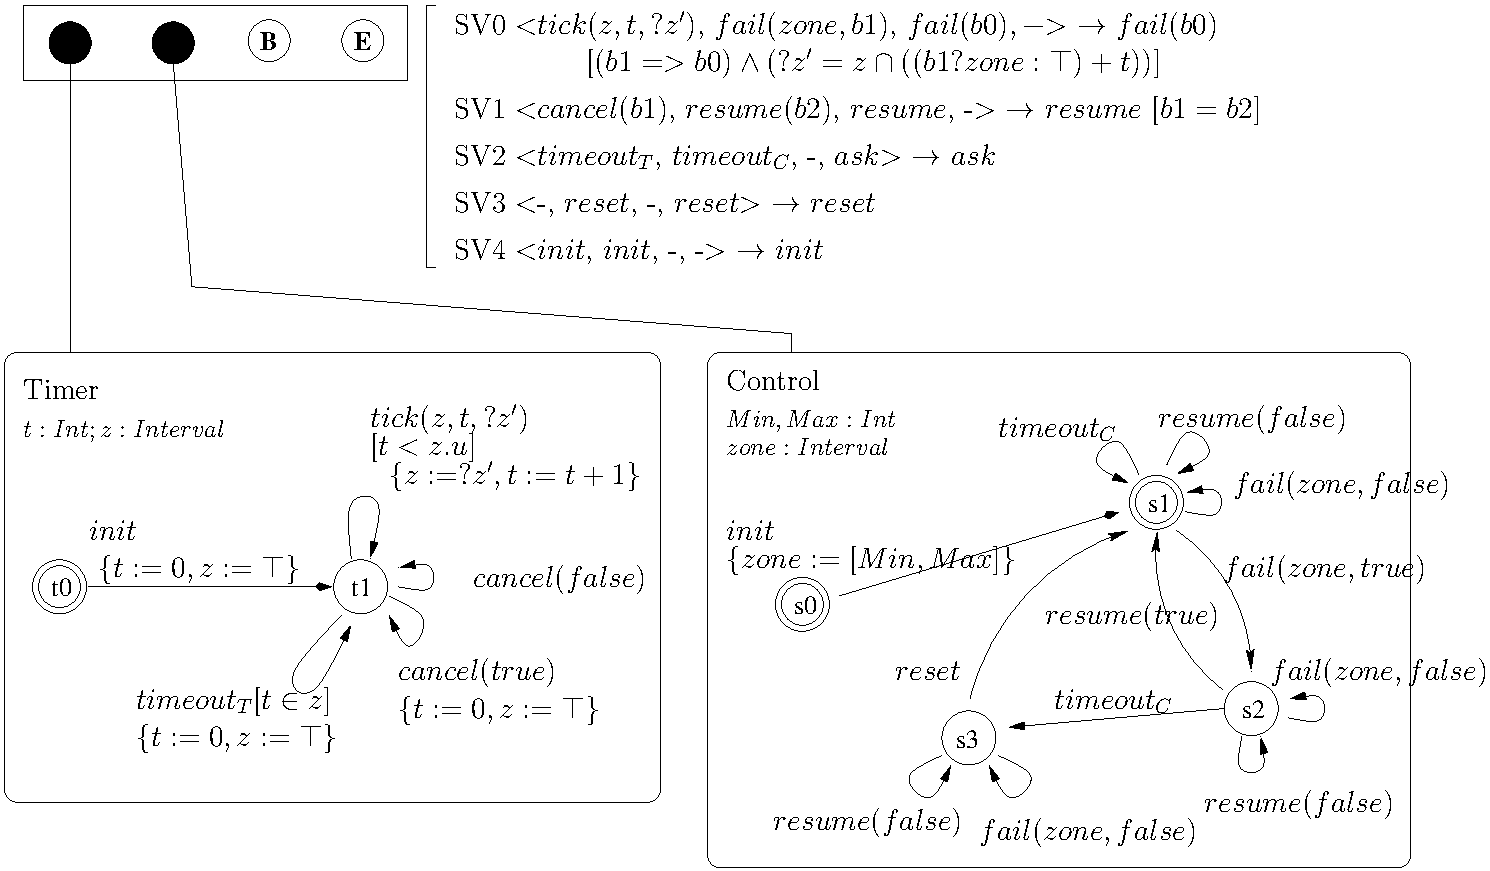
\includegraphics[width=0.9\columnwidth]{XFIG/FailureTimerPNET-v4}
  \caption{The open pNet encoding the Failure Monitor architecture (\ref{fig:schema:ArchFailure:BIP}) without the Max Progress priority model}
  \label{fig:FailureTimer:pNet}
\end{figure}

\begin{figure}[t]
  \centering
  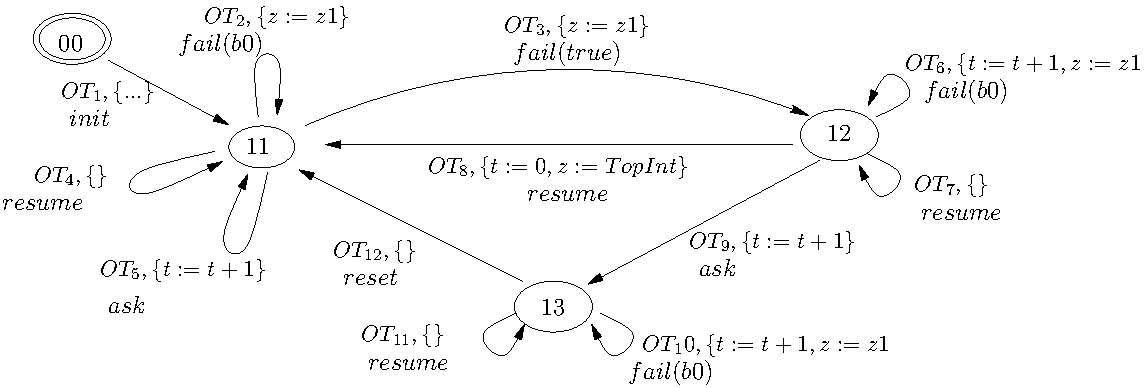
\includegraphics[width=0.9\columnwidth]{XFIG/TimerOADetailed}
  \caption{The open Automaton of the Failure Monitor Architecture}
  \label{fig:ArchFailure:OA}
\end{figure}

Figure \ref{fig:ArchFailure:OA} shows the open automaton built by our
algorithm. For reasons of readability, we did not show the full
details of the open transitions on this figure. Below we list the
first 3 of them (full details available in \ref{TimerRR}). 
This automaton has 12 transitions, including those encoding various
possible firing of some interactions (e.g. OT 2 and 3 for
{\PortFail}). It looks like the rough behaviour is
reasonable, although a detailed study shows that the property stated
above does not hold, because of the
{\PortFail} loops on states $11$ and $12$. This is because we did not
use the maximal progress assumption here. If we do, we get the
corrected behaviour in Figure \ref{fig:ArchFailure:OA-MaxProgress}, in
which $OT_7$ has disappeared, and $OT_2$ and 
$OT_{10}$ have been restricted to $b0=\false$.

\bigskip
\noindent
$  OT_1  = \openrule
{\emptyset, \{t:=0, z:=TopInt, zone:=[minZone,maxZone]\} }
{\ostate{00} \OTarrow{init} \ostate{11}}
$

\medskip    
\noindent
$  OT_2  = \openrule
{\{B\mapsto fail(b0)\},\\
  t<GetMax(z) \land b1=false \land b1=>b0 \land z1= (z \cap (b1?zone;TopInt)+t),\\
  \{z:=z1\} }
{\ostate{11} \OTarrow{fail} \ostate{11}}
$
\medskip
  
\noindent
  $  OT_3  = \openrule
  {\{B\mapsto fail(b0)\},\\
    t<GetMax(z) \land b1=true \land b1=>b0 \land z1= (z \cap (b1?zone;TopInt)+t),\\
    \{z:=z1\} }
  {\ostate{11} \OTarrow{fail} \ostate{12}}
  $
  \medskip


  \begin{figure}[t]
  \centering
  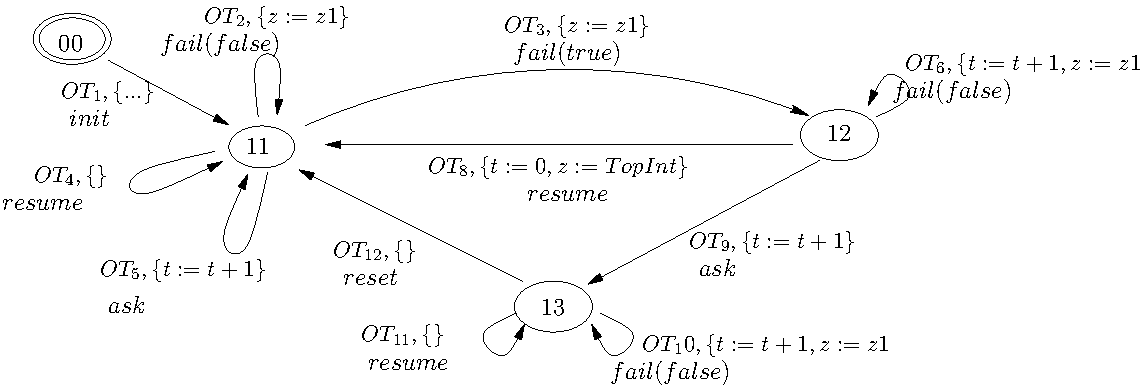
\includegraphics[width=\columnwidth]{XFIG/TimerOAMaxProgress}
  \caption{The open Automaton of the Failure Monitor Architecture,
    with Maximal Progress}
  \label{fig:ArchFailure:OA-MaxProgress}
  \end{figure}

  \TODO{Eric: Explain}
\begin{itemize}
\item $OT_2$ and $OT_{10}$ have changed because $b0=true$ is no longer possible
\item $OT_7$ has disappeared because it is now unsat.
\end{itemize}


\subsection{Benefits from the Smart algorithm}

In each cell of the following table, we display the number of OTs whose predicates were founSAT/UNSAT by the SMT engine, and the overall time spent for the whole algorithm execution.

	\begin{tabular}{p{4cm}p{3cm}p{3cm}}
		\hline\specialrule{0em}{1pt}{1pt}
		Use-case & Brute force & Smart algorithm
                \\\specialrule{0em}{1pt}{1pt}
		\hline\specialrule{0em}{3pt}{3pt}
		Enable operator   			&
                5/55 OTs           &
                5/42 OTs
                \\\specialrule{0em}{1pt}{1pt} 

                ``(P>Q)>R'' 		&
                376 ms 				&
                344 ms  
		\\\hline\specialrule{0em}{3pt}{3pt}
		SimpleProt    			&
                7/260 OTs           &
                7/57 OTs
                \\\specialrule{0em}{1pt}{1pt} 

                (no holes)&
                1536 ms 				&
                359 ms  
%                \\\specialrule{0em}{1pt}{1pt}
%                \textsl{for any sort} & & $=,\ \ne$
		\\\hline\specialrule{0em}{1pt}{1pt}
		SimpleProt    			&
                19/836 OTs           &
                19/185 OTs
                \\\specialrule{0em}{1pt}{1pt} 

                (with 2 client holes)&
                2496 ms 				&
                844 ms  
		\\\hline\specialrule{0em}{1pt}{1pt}
		FailureTimer    			&
                12/235 OTs           &
                12/180 OTs
                \\\specialrule{0em}{1pt}{1pt} 

                (no Max Progress)&
                1253 UNSAT           &
                812 UNSAT
                \\\specialrule{0em}{1pt}{1pt}
		&
                1253 ms 				&
                812 ms  
		\\\hline\specialrule{0em}{1pt}{1pt}
		FailureTimer X 2    			&
                37/3136 OTs           &
                37/2416 OTs
                \\\specialrule{0em}{1pt}{1pt} 

		&
                8923 ms 				&
                6798 ms  

		\\\hline
	\end{tabular}

        This shows a significant benefit of the ``smart'' strategy, in the considered use-cases, between 30 to 60\% gain depending on the examples.

\section{Conclusion and Discussion}
\label{section:conclusion}

The formal definitions and properties of the open pNets model were
published in \cite{henrio:Forte2016}. In this new work we describe an implementation of
the model and its semantics construction, including its interaction
with the Z3 SMT engine.
The implementation has two parts: the first is a finitary algorithm
that builds all possible combinations of synchronisations through the
pNet hierarchical structure. The result is a so-called
\emph{open-automaton}, which transitions contains predicates relating
the actions of the pNet holes and controllers. Some of the open
transitions obtained at this step,  may
contain predicates which do not represent any possible concrete
instantiations. 
In the second part of the tool we use the SMT solver Z3 for checking the
satisfiability of the predicate in each open transition. 
To this end, we encode into Z3 the representations of the action algebra and
the predicates before submitting them to the
Z3 solver. 
%
%\hl{%
%
In this paper, we used a running example, based on a BIP
architecture from an earlier nanosatellite case
study~\cite{CubETH-case-study}.  This example shows that
open-automata-based semantics can be instrumental in verifying the
properties enforced by the architectures through an encoding into open
pNets.  This encoding\mdash which we intend to formalise and prove
correct in a separate paper\mdash also opens the way for an extension
of BIP architectures with the transfer of data among variables of
different components.  Indeed, such data transfer can be easily
encoded using the predicates associated to synchronisation vectors in
open pNets.  The encoding of open transitions into SMTlib and the
availability of theories can guide the definition of such an extension.
%
%}
%
Our case-studies show that our encoding
successfully identifies the unsatisfiable open transitions and that
the resulting automata correctly reflect the expected 
movements of the encoded process expressions.   

%% Among the questions that have arised during this work, an important one is the
%% efficiency of Z3 for our needs. Z3 is famous for being very fast in
%% solving very large sets of assertions. %% , which could be important for
%% %% us
%% However, we encountered problems during the implementation of the
%% checking method. %% using Z3. 
%% For example, if the $\mathit{functions}$ and the
%% $\mathit{datatypes}$ part of the algebra presentation that we submit to the solver
%% are independent from each other, then checking the $\mathit{assertions}$ is 
%% simple. However, $\mathit{functions}$ on recursive $\mathit{datatypes}$ make it
%% more complex. Special rules might be defined by the user for the
%% induction.  We need more evidence that dealing with more complex
%% action algebras, which would involve axiomatizing their data structures
%% as Z3 theories, will allow us to decide validity of
%% predicates.
%% We may also try other automatic theorem provers, depending on the structure of the proofs we need.

%% \todoMargin{Change perspective: we are working on the formal extension of
%%   BIP architectures, and their semantics in terms of pNets. Then
%%   bisimulation and model-checking principles adapted to open pNet
%%   systems are under development}
%
Naturally, our next goals after the generation of the open automata
will be to model-check logical properties, and to check equivalence of pNets. While
model-checking open automata  seems easy to define, equivalence
checking is more challenging. 
In~\cite{henrio:Forte2016}, we
have already found the FH-bisimulation, %inspired
%by~\cite{deSimone85},
to be a
suitable definition. But weak equivalences, or refinements, will
definitely be useful when comparing different pNets with
different structure. For bisimulation, we foresee that SMT methods
will be the basis for comparison of open transitions. 
%However, the usual approach of computing bisimulation by partition
%% refinement does not work easily with symbolic transitions. In a first
%% step we may want instead to define and implement an algorithm for
%% checking that a given equivalence relation between open automata 
%% states is indeed a FH-Bisimulation. Finding automatically a
%% bisimulation relation or the most general bisimulation will be more
%% challenging.
%% It appears also that when comparing different pNets with
%% different structure, strong bisimulation will be too strong a notion,
%% and that we will have to define proper notions of weak equivalence or
%% refinements. 

\emph{Scaling up.} One important motivation of this work is to
attack the complexity of verification of realistic systems by a
compositional and parametric approach. Still one may wonder if the price
for analysing our symbolic transitions will not make the approach too expensive
in term of computing time. We tried a
slighly bigger example, assembling 2 Failure controllers. In~\cite{Avocs-RR}, we show that Z3 can check the
satisfiablility of a 90K open transitions in a couple of minutes.



\bibliographystyle{spmpsci}

% \bibliography{oasis,biblio}
\bibliography{biblio}



\end{document}

%\newpage
\appendix
\section{Changes from pre-proceedings version}
All minor requests from reviewers (typo, grammar) were already corrected in the preproceedings version.

Request from Reviewer 3, that we had not done in the preproceedings, for matter of space, have now been shortly answered.
More precisely,
\begin{itemize}
\item{} in section \ref{section:op-semantics}, we have added a precise statement of our finiteness theorem, that answers the question about termination of the algorithm.
\item{-} in section \ref{section:pruning} we have added more explanations about the way that various data types theories will be handled by the SMT engine
\end{itemize}


The following appendices are included for the convenience of reviewers.
Our intention is to publish as a research report, before final publication, an
extended version containing all technical details, proofs, and more examples.

The appendices are organized in the following way:

\begin{enumerate}
\item[A] pNet semantic rules
\item[B] Variable management
  \subitem B.1 fresh variables
  \subitem B.2 managment of state variables
\item[C] Algebra presentations
\item[D] Well-formness and typing of expressions
\item[E] Translation to SMTlib input language
\item[F] Full output for the FailureTimer open automaton
\item[G] Scaling up
  
\end{enumerate}


\section{pNet semantic rules}
\label{appendix:semRules}

\paragraph{Note:} For convenience, we have included here the semantic rules for pNets,
that were already published in \cite{henrio:Forte2016}.

We build the semantics of an open pNet as an open automaton where
LTSs are the pLTSs at 
the pNet leaves, and the states are structured as in
the previous section. 
%given by Definition~\ref{def-states}.
To build an open transition one first
 projects the global state into states of the leaves, then applies
pLTS transitions on these states, and compose them with actions of
holes using synchronisation vectors. %The pNet
%structure does not appear in the open-automaton, only the
%set of Holes and the set of Leaves.

The semantics   regularly instantiates \emph{fresh} variables, and uses a
\emph{clone} operator that clones a term replacing each variable with a
fresh one.
The variables in each synchronization vector are considered local:
for a given pNet expression, we must have fresh local variables for
each occurrence of a vector (= each time we instantiate rule
Tr2). Similarly the state variables of each copy of a
given pLTS in the system, must be distinct, and those created for each
application of Tr2 have to be fresh and all distinct. 

% The semantic of the open pNets is already defined as an open automaton
% in \cite{henrio:Forte2016} using open transitions to present the
% transitions of its global states.

\begin{definition}[Operational semantics of open pNets]
  \label{def:operationalSemantics}
  The semantics of a pNet $p$ is an open automaton $A = <Leaves(p),J,\mathcal{S}, s_0,
  \mathcal{T}>$ where:
  \begin{itemize}
    \item $J$ is the indices of the holes: $Holes(p)= H_j^{j\in J}$.
    %  \item $\overline{L}^L = Leaves(p), \overline{H}^J = Holes(p)$
    \item $\overline{\mathcal{S}} = States(p)$ and $s_0 = InitState(p)$
    \item $\mathcal{T}$ is the smallest set of open transitions
    satisfying the rules below:
  \end{itemize}
  
  The rule ({\bf Tr1}) for a pLTS $p$  checks that the guard 
  is verified and transforms assignments into post-conditions:
  
  \begin{description}
    \item[{\bf Tr1:}]
    $\inferrule
    { s \xrightarrow{\langle \alpha,~e_b,~(x_j\!:= {e}_j)^{j\in
          J}\rangle} s'\in \to  \\
      {\tt fresh}(v) \\
      Pred = ~e_b \land (v = \alpha)
    }
    { p = \mylangle  S,s_0, \to \myrangle
      \models
      \inferrule*[myfraction=\reddottedrule]
      {\{s \xrightarrow{\alpha}_p s'\} ,\emptyset ,
      Pred,\left\{x_j\gets e_j\right\}^{j\in J}}
      {\ostate{s} \xrightarrow{v} \ostate{s'}}
    }
    $
  \end{description}
% Note that this note is greatly simplified by the fact that variables are local to 
% thread; introducing global state variables or accepting loops to the same 
% state would 
% require to reason 
% on the scope of 
% each variables, and to introduce additional variables to handle the several occurence 
% of the same pLTS variable in the predicates. Indeed the constraints on pLTS 
% transitions 
% ensure that the same variable never appears both on the left and on the right of the 
% equations of a predicate.
  
  The second rule ({\bf Tr2}) deals with pNet nodes: for each possible
  synchronization vector applicable to the rule subject, the premisses
  include one {\em open transition} for each sub-pNet involved, one possible
  {\em action} for each Hole involved, and the predicate relating these
  with the resulting action of the vector.
  A key to understand this rule is that the open transitions are
  expressed in terms of the leaves and holes of the pNet structure,
  i.e. a flatten view of the pNet: e.g. $L$ is the index set of the
  Leaves, $L_k$ the index set of the leaves of one subnet, so all $L_k$
  are disjoint subsets of $L$. % Thus the states in the open transitions,
%   at each level, are tuples including states of all the
%   leaves of the pNet, not only those involved in the chosen
%  synchronization vector.
  
  \begin{description}
    \item[{\bf Tr2:}]
  \end{description}
  
  \noindent
    $\inferrule
    {k\!\in\! K \\ SV\!\!= \!clone(SV_k) \!=\! \alpha_m^{m \in I_k\uplus J_k} \!\to\! 
    \alpha'_k, G_k \\
      Leaves(p) \!=\! \pLTS_l^{l\in L} \\     
      \forall m\in I_k.
      \pNet_m \models
      \inferrule*[myfraction=\reddottedrule]
      {\{s_{i}\xrightarrow{a_{i}}_i s_{i}'\}^{i\in I_m^\prime},
      \{\xrightarrow{b_{j}}_j\}^{j\in J'_m}, \Pred_m, \Post_m}
      {\ostate{s_{i}^{i \in L_m}} \xrightarrow {v_m}
        \ostate{s_{i}^{\prime\ i \in L_m}}}
      %\land
      %Leaves(\pNet_m) = \overline{pLTS}^{L_k})
      \\
      I' = \biguplus_{m\in I_k}\!\! I_m'
      \\ J' = \biguplus_{m\in I_k}\!\! J'_m \uplus J_k  \\
      \Pred = \bigwedge_{m\in I_k}\!\! \Pred_m \land
      \MkPred(SV,v_m^{m\in I_k},b_j^{j\in J_k},v)\\
      \forall j\!\!\in\!\! J_k. {\tt 
        fresh}(b_j) \\ {\tt fresh}(v) \\ 
      \forall i\in
      L\backslash I'.\,s'_i=s_i 
    }
    {p = \mylangle \pNet_i^{i\in I}, S_j^{j\in J}, \symb{SV}_k^{k\in K}\myrangle
      \models
      {\inferrule*[myfraction=\reddottedrule]
        {\{s_i\xrightarrow{a_i}_i s_i^{\prime}\}^{i\in I^\prime},
        \{\xrightarrow{b_j}_j\}^{j\in J^\prime}, \Pred, \uplus_{m\in I_k} 
        \Post_m}
        {\ostate{s_i^{i\in L}} \xrightarrow {v}
          \ostate{s_i^{\prime i\in L}}}
      }
    }
    $

  \medskip  
\end{definition}

In rule TR2, the generated predicate is composed of the conjunction of
the predicates of the subnets' OTs, with the additional part encoding
the application of the chosen synchronisation vector.
In \cite{henrio:Forte2016} this last part is defined as:
\[\MkPred(SV_k, a_i^{i\in I}, b_j^{j\in J}, v)\Leftrightarrow
\begin{array}{l}
\exists {(a'_i)}^{i\in I},
{(b'_j)}^{j\in J},v'.\, SV_k={(a'_i)}^{i\in I}, {(b'_j)}^{j\in J}\rightarrow v'
\\~~\land
\forall i\in I.\, a_i=a'_i\land \forall j \in J.\, b_j=b'_j \land v=v'
\end{array}\]

%% This definition is not constructive, but the existentialy quantified
%% variable sets here correspond the subsets of subnets and holes that
%% are effectively involved in vector $SV_k$.
%% Within our algorithm, these subsets have been computed by $Combining$ and
%% passed as arguments to the $Matching$ method, so
%% we can construct this predicate fragment as:

%% \[\Pred(SV, \overline{\pNet},\overline{S}, v) = 
%% \begin{array}{l}
%% \forall {(a'_i)}^{i\in I},
%% {(b'_j)}^{j\in J},v'.
%% \\
%% v_m=a'_i\land \, b_j=b'_j \land v=v' \land G_k
%% \end{array}\]
%% \TODO{Eric: to be checked}

Within our algorithm, these subsets have been computed by the
$Combining$ method and passed as arguments to the $Matching$ method
(see section~\ref{section:implementation}) 

\paragraph{Termination.} To have some practical interest, it is important to know when this
algorithm terminates. The following theorem shows that an open-pNet
with finite synchronization sets, finitely many leaves and
holes, and each pLTS at leaves having a finite number of states and
(symbolic) transitions, has a finite automaton. The proof can be found
in \cite{henrio:Forte2016}. 


\begin{theorem}[Finiteness of open-automata.]\\
Given an open pNet $pnet=\mylangle \overline{\pNet},\overline{S}, \symb{SV}_k^{k\in K}\myrangle$ with leaves $l_i^{i\in L}$ and holes $h_j^{j\in
  J}$, if the sets $L$ and $J$ are finite, if the synchronization vectors of all pNets 
  included in  $pnet$ 
  are finite, and if
$\forall i \in L.\, finite{(states(l_i))} \text{ and } l_i$
has a finite number of state variables, then Algorithm 1 terminates
and produces an open automaton 
$\mathcal{T}$ with finitely many states and transitions.


Given an open pNet $\mylangle \overline{\pNet},\overline{S}, \symb{SV}_k^{k\in
    K}\myrangle$ with leaves $pLTS_i^{i\in L}$ and holes $Hole_j^{j\in
  J}$,
build its semantics as in algorithm 1.

We have:

$$ finite{(L)} \land finite{(J)} \land \forall i \in L finite{(\{s_i\})}
  \to finite{(\mathcal{T})}$$
\end{theorem}


\section{Variable management}
In this section we give more details on two facets of variable
management in the tool: the generation of variables names, and the
management of state variable assignments.

\subsection{Fresh variables}
\label{appendix:variables}
The variables in each synchronisation vector are considered local: for
a given pNet expression, we must have fresh local variables for each
occurrence of a vector (= each time we instantiate rule
Tr2). Similarly the state variables of each copy of a given pLTS in
the system, must be distinct, and those created for each application
of Tr2 have to be fresh and all distinct. This will be implemented
within the open-automaton generation algorithm, e.g. using name
generation using a global counter as a suffix.

Application of the semantic rules require generating a lot of fresh
names, for different kind of variables. We could use a global name
generator to guarantee unicity, but 
at the same time, we also hope them still
readable. Here we rename the variables with a regular format using the fresh function.
More precisely, the fresh function generates a new name adding a
suffix after the original name. The suffix contains three parts
combined by a colon.  


\begin{definition}[Fresh variable]\label{fresh-variable}
The format of \emph{fresh variable} (renaming) is defined as:
``$\emph{prefix : tree\ index\ :\ counter}$''.
\begin{itemize}
   \item[$\bullet$] $prefix$ identifies the kind of the
     variable. Current kinds are: sva\_<SV> (action variable in vector
     $SV$), ra (result action), hb\_<B> (behaviour of hole $B$).
   \item[$\bullet$] $tree\ index$ is the index of the node containing
     the variable in the tree-like structure of the pNet. 
   \item[$\bullet$] $counter$ is the current value of the corresponding counter.
\end{itemize}
\end{definition}

%\TODO{Option: Add the process and the vector ids ?}

%$Prefix$ avoids the confusion between variables from different structures with the same name by attaching the type of the structure. $Tree\ index$ is given to every node of the pNets to mention which node the variable belongs to as pNets has a tree-like structure. To each node, the tree index is always a number sequence of the tree index of its higher level and the index of the node in this level at the last. $A\ set\ of\ counters$ is used to count the current times the SV, Hole, subnet invoked, or the number of possible OT generated to provide an identity. 

For example, in the running example, in the raw output listing in
Appendix~\ref{appendix:fullOutput}, in the first OT, you find variables: 
\begin{itemize}
   \item $\OTvar{:hb\_B:13:1}$ that is the behaviour of hole ``B''
   \item $\OTvar{b1:sva\_SV0:1:1}$ variable ``b1'' from vector ``SV0''
   \item $\OTvar{:ra:1:1}$ result action of the current OT
\end{itemize}

\subsection{Management of state variables}
\label{appendix:translating-assignments}
In a pLTS, there may be several incoming transitions 
that assign potentially different values to a state variable.
To handle such cases, the algorithm manages for each pLTS state, as a
list of expressions collected from the assignments of each state
variable $v$ (as registered in the incoming OTs).
%% The list we used contains triples <$v$, $S$, $AssignRH$> 
%% where $v$ is the variable in pLTS, $S$ is its owner state and
%% $AssignRH$ is a list of expressions over other variables in the right
%% hand side of assignments of $v$.
% As a pragmatic extension to the formal definition, we also manage
% ``global variables'', defined in all states of the pLTS.
For a global state in the open automaton, getting the set of state
variables (which may be used in a transition) will simply be the union
of state variables of the individual pLTS states constituting this
global state, as variables of different pLTS are distinct.

 We define:
\begin{itemize}
  \item $SVars(gs)$ the state variables of all states in the global
    state $gs$
  \item $Assigns(svar)$ the set of possible assignments of variable
      $svar$.
\end{itemize}
These will be used when translating the predicates into SMTlib
language.


\section{Algebra presentations}
\label{appendix:algpresentations}
In order to submit satisfiability problems to Z3 (for the predicates
in open transitions), we need to generate SMTlib programs, from the
pNet Algebra presentation and predicates.
More precisely, we need to translate to SMTlib:
\begin{itemize}
  \item the presentation of the action algebra
    (sorts and operators) that is defined for a given language (process calculus, or high level programming language),
    \item for a given pNet, the set of local constants (actions or auxiliary data) that are used in the pLTSs,
    \item for each open transition: the declaration of variables, and
      the predicate (including action expressions).
\end{itemize}

During this translation, in order to guarantee that the generated code
will cause no runtime errors during parsing and execution, we need
to ensure that all objects used in the SMTlib code are properly
declared, and that they are correctly typed.

Note that in principle, an action algebra corresponds to a given
high-level language (e.g. a process algebra), and that the algebra
presentation will be defined once and for all in the framework of the
pNet semantics of each specific language.

\subsection{Definition of an algebra presentation}
We have a minimal, predefined algebra presentation for all pNets, including
three basic sorts $Bool$, $Action$ and $Int$ and their
operators. Table \ref{Table:predefinedSorts} defines these elements.

In addition, and for convenience, we provide one generic construct for
parameterized actions named FUN, which can accept any number of
arguments of any sort. The result type, though, can only be $Action$,
in order to keep the type-checking simple (see next section).

\begin{table}\caption{\label{Table:predefinedSorts}\leftline{Algebra Presentation: predefined Sorts
  and Operators}}
	\begin{tabular}{p{3cm}p{3cm}p{6cm}}
		\hline\specialrule{0em}{1pt}{1pt}
		Sort & Constructors & Auxiliary Operators
                \\\specialrule{0em}{1pt}{1pt}
		\hline\specialrule{0em}{3pt}{3pt}
		Bool    			&
                $\texttt{true},\ \texttt{false}$&
                $\land,\ \lor,\ \neg,\ \implies$
                \\\specialrule{0em}{1pt}{1pt} 
		Action 			&  $\texttt{FUN}$ &
                \\\specialrule{0em}{1pt}{1pt}
		Int 				&
                ${0, \{i, -i\}_{i \in \texttt{Nat}}}$  &
                $- \texttt{(unary)},\ +,\ -
                \texttt{(binary)},\ \times,\ \div, \texttt{etc.}$
                \\\specialrule{0em}{1pt}{1pt}
                \textsl{for any sort} & & $=,\ \ne$
		\\\hline
	\end{tabular}
\end{table}

\begin{table}\caption{\label{table:BIPoperators}\leftline{Additional
      operator for the BIP algebra}}
	\begin{tabular}{p{3cm}p{3cm}p{6cm}}
		\hline\specialrule{0em}{1pt}{1pt}
		Sort & Constructors & Auxiliary Operators
                \\\hline\specialrule{0em}{1pt}{1pt} 
		Action 			&  $\texttt{FUN\_Action\_Bool}$ &
		\\\hline
	\end{tabular}
\end{table}

For a given language, or for a given use-case, the designer can
declare more sorts and operators, using our pNet API.
As an example, a (value-passing) CCS action algebra, where we assume a
single auxiliary value domain ``Data'', can be defined as:

\begin{example}
  \label{example:CCSpresentation}
  \begin{itemize}
    \item[]
    \item $Sorts_{CCS} = \{Action, Channel, Data, Int, Bool\}$
    \item $Constrs_{CCS} =\\
    \texttt{Emit}: 2, \{(Chan\_E:Channel),(Value\_E:Data)\}->Action\\
    \texttt{Receive}: 2, \{(Chan\_R:Channel),(Value\_R:Data)\}->Action\\
    \texttt{Tau}: 0, \{\}-> Action\\
    \texttt{... and all predefined operators}$
  \end{itemize}
\end{example}

\begin{table}\caption{\label{table:CCSalgebra}\leftline{Additional
      sorts and operators for the CCS algebra}}
	\begin{tabular}{p{3cm}p{3cm}p{6cm}}
		\hline\specialrule{0em}{1pt}{1pt}
		Sort & Constructors & Auxiliary Operators
                \\\specialrule{0em}{1pt}{1pt}
		\hline\specialrule{0em}{3pt}{3pt}
		Channel, Data    			&
                $\emptyset$&
                $\emptyset$
                \\\specialrule{0em}{1pt}{1pt} 
		Action 			&  $\texttt{Emit(c,v)},\texttt{Receive(c,v)},\texttt{Tau}$ &
		\\\hline
	\end{tabular}
\end{table}


Then in pNet API these operators or constants can be declared as:
\begin{lstlisting}[basicstyle=\scriptsize\ttfamily, language=java, frame=single]
AlgebraSort Action = new AlgebraSortImpl("Action");
AlgebraSort Channel = new AlgebraSortImpl("Channel");
AlgebraSort Data = new AlgebraSortImpl("Data");
Action.addConstructor("Emit", {"Chan_E", "Value_E"}, {Channel, Data});
Action.addConstructor("Receive", {"Chan_E", "Value_E"}, {Channel, Data});
Action.addConstructor("Tau");
\end{lstlisting}

%\subsection{Constants and variables in pNets and in open transitions}
\subsection{Extended presentation, and Environment}

In addition to the objects defined in the Algebra Presentation, there are
specific objects that are introduced by the pNet construction, and by
the semantic rules used to build the open transitions and their
predicates. This includes, for a pNet $pnet$
\begin{itemize}
\item $Const(pnet)$: Constants from the pLTSs (controllers) transitions: these are
  new constant constructors, usually of sort Action, local to an
  instance of a controller. The pNet definition requires that all
  these constants are distinct from each other.
\item $SVars(pnet)$: State variables of the controllers. Here also they are required
  to be distinct from those of other controllers.
\item $IVars(pnet)$: Input variables of the controllers.
\item $FVars(pnet,ot)$: Several kinds of ``fresh'' variables, created by application of
  rule Tr2, during the construction of each open transition $ot$:
  Action variables for the behaviour of holes and the 
  resulting actions of transitions, variables created during the cloning
  of synchronisation vectors.
\end{itemize}

\def\EPres{\mathcal{P}}
\def\EEnv{\Gamma}

All variable sets above include their sort.
To define the typing rules for expressions and the translation
functions, for any pNet $pnet$ and open transition $ot$, we define an
extended presentation $\EPres_{pnet}$ and environment $\EEnv_{pnet,ot}$ that includes all of the
objects above:

\begin{definition}
  Given an algebra presentation $\APres_{pnet}=<Sorts,Constrs,Ops>$ and a pNet $pnet$, we
  construct:
  \begin{itemize}
  \item An extended presentation $\EPres_{pnet}<Sorts,Constrs \cup Const(pnet),Ops>$.
  \item For a given open transition $ot$, an environment
    $\EEnv_{pnet,ot}=SVars(pnet) \cup IVars(pnet) \cup FVars(pnet,ot)$. 
  \end{itemize} 
\end{definition}



\section{Well-formness and typing of expressions}

The purpose of this section is to define static semantic notions that
will guarantee that the translation to the SMT language will be
correct, i.e. will not yield errors at runtime. This includes
well-formness (all sorts, operators, variables are defined, and
expressions respect the arity of operators), and typing rules.
%\TODO{Eric: refer in the appendix header}

\begin{definition}
  Given a presentation $\EPres$ (possibly extended) and an environment $\EEnv$:
  \begin{itemize}
  \item $\EEnv$ is well-formed if all sorts in $\EEnv$ are
    defined in $\EPres$
  \item an expression is well-formed if all its operators are defined
    in $\EPres$, and used with the proper arity, and all its
    variables are defined in $\EEnv$
  \item an expression is well-typed if it can be typed by the typing
    rules in table \ref{table:typing-rules}
  \end{itemize}
\end{definition}

The following judgment, and the typing rules in table
\ref{table:typing-rules} can be used to check both the wellformedness
and well-typing of expressions in a pNet or in an open transition,
given the corresponding $\EPres$ and $\EEnv$.

%\begin{table}\caption{\leftline{Typing judgment for Expressions in Open pNets}}
\vspace{1ex}
\noindent
\begin{tabular}{p{5cm}p{7cm}}
		\hline\specialrule{0em}{3pt}{3pt}
%%		$\EEnv \vdash \diamond$ 					& $\EEnv$ is a well-formed environment 					\\\specialrule{0em}{1pt}{1pt}
%%		$\EEnv \vdash A$ 							& A is a well-formed type in $\EEnv$	 					\\\specialrule{0em}{1pt}{1pt}
		$\EPres,\EEnv \vdash M: A$
                & M is a well-formed term of type A in $\EPres,\EEnv$			\\\specialrule{0em}{1pt}{1pt}
		\specialrule{0em}{3pt}{3pt}\hline
	\end{tabular}
%\end{table}	

\begin{table}\caption{\leftline{Type Rules for Open pNets}}
  \label{table:typing-rules}
	\begin{tabular}{p{5cm}p{5cm}p{2.5cm}}
		\hline\specialrule{0em}{3pt}{3pt}
		%% (Env $\varnothing$) 								
		%% & 										
		%% &					\\\specialrule{0em}{1pt}{1pt}
            %% $\dfrac{ }{\varnothing \vdash \diamond}$			
            %% & %$\dfrac{\EEnv \vdash A ~~ x\ }{\varnothing \vdash \diamond}$
            %% &					\\\specialrule{0em}{3pt}{3pt}
		%% (Type Bool) 										
		%% &(Type Action) 						
		%% &(Type Int)			\\\specialrule{0em}{1pt}{1pt}
		%% $\dfrac{\EPres \vdash Bool~~\EEnv \vdash \diamond}{\EPres,\EEnv \vdash Bool}$ 
		%% & $\dfrac{\EPres \vdash Action~~\EEnv \vdash \diamond}{\EPres,\EEnv \vdash Action}$ 
		%% & $\dfrac{\EPres \vdash Int~~\EEnv \vdash \diamond}{\EPres,\EEnv \vdash Int}$        \\\specialrule{0em}{3pt}{3pt}
		(Var x) 										
		& 						
		&			\\\specialrule{0em}{1pt}{1pt}
		$\dfrac{\EEnv \vdash x:A}{\EPres,\EEnv \vdash x:A}$ 
		&  
		&       		\\\specialrule{0em}{5pt}{5pt}
		\multispan{2} (Binary operators, e.g.: $\land, \lor$ for Booleans, $+, -, \times, \div, \le, \ge$ for integers, etc.)								
							
		& 			\\\specialrule{0em}{3pt}{3pt}
		$\dfrac{\EPres \vdash BinOp :: ty1, ty1 \rightarrow ty2 ~~\EEnv \vdash x_1:ty1 ~~\EEnv \vdash x_2:ty1}{\EPres,\EEnv \vdash x_1 ~BinOp~ x_2:ty2}$ 
		& 
		&       		\\\specialrule{0em}{3pt}{3pt}
		\multicolumn{2}{l}{(Unary operators, e.g. $\lnot$ for Booleans, - for integers)}	
                
		& 			\\\specialrule{0em}{3pt}{3pt}
		$\dfrac{\EPres \vdash UnOp :: ty1 \rightarrow ty2 ~~\EEnv \vdash x:ty1}{\EPres,\EEnv \vdash Unop~x:ty2}$   
		&&       		\\\specialrule{0em}{5pt}{5pt}
		(Polymorphic EQ and NEQ)							
		&					
		&
                                         \\\specialrule{0em}{3pt}{3pt}
		$\dfrac{\EPres \vdash A  ~~\EEnv \vdash x_1:A ~~\EEnv \vdash x_2:A}{\EPres,\EEnv \vdash x_1 = x_2:Bool}$ 
		& 
		$\dfrac{\EPres \vdash A  ~~\EEnv \vdash x_1:A ~~\EEnv \vdash x_2:A}{\EPres,\EEnv \vdash x_1 \ne x_2:Bool}$ 
		
		&       		\\\specialrule{0em}{5pt}{5pt}
		(Overloaded FUN operator)							
		&					
		& 			\\\specialrule{0em}{3pt}{3pt}
		$\dfrac{\EPres \vdash \texttt{FUN} :: A_1,...,A_n \rightarrow Action ~~\EPres \vdash A_1~~...~~\EPres \vdash A_n ~~\EEnv \vdash x_1:A_1~~...~~\EEnv \vdash x_n:A_n}{\EPres,\EEnv \vdash \texttt{FUN}(x_1,...,x_n):Action}$ 
		& 
		&			\\
		\specialrule{0em}{5pt}{5pt}\hline
	\end{tabular}
\end{table}	

\begin{remark}
  These rules provide a simple type-checking algorithm: if all
  variables in an expression are known in $\EEnv$, then a bottom-up
  application of the rules will decide whether the expression is
  well-typed, and compute the type of each sub-expression.
\end{remark}


\section{Translation to SMTlib input language}
\label{appendix:mapsmt}
The pNet elements, as defined above, can be full translated into
SMT-LIB language (\cite{BarFT-RR-17}), but there are a number of differences in the
structure of the models/languages, so the translation is not trivial.

In this section we define separately
\begin{itemize}
\item The translation of the
extended algebra presentation for one pNet (so it will be common for
the study of all OTs of one use-case);
\item and the translation of each open transition of the pNet,
  including its environment (list of variables), its predicate, and
  the encoding of the possible values of the state-variables of its
  source global state.
\end{itemize}
The following table summarizes the main elements of the translation.

\def\translate{~\lhook\joinrel\longrightarrow}

\vspace{1ex}\noindent
%\begin{table}\caption{\leftline{Mapping}}
	\begin{tabular}{p{3cm}p{9cm}}
		\hline\specialrule{0em}{1pt}{1pt}			
		(Presentation)							
		&								\\\specialrule{0em}{1pt}{1pt}		
		&$Sorts \& Constructors \translate$	declare-datatypes				\\\specialrule{0em}{1pt}{1pt}
		&$Other operators \lhook\joinrel\longrightarrow$	declare-function		\\\specialrule{0em}{1pt}{1pt}
		(Open Transition)							
		&								\\\specialrule{0em}{1pt}{1pt}
		&$\EEnv ~~\lhook\joinrel\longrightarrow$	declare-const		\\\specialrule{0em}{1pt}{1pt}
		&$Pred ~~\lhook\joinrel\longrightarrow$	 assert		\\\specialrule{0em}{1pt}{1pt}
%		&$\texttt{FUN}(x_1,...,x_n)$	\TODO {Xudong, why ?}	\\\specialrule{0em}{1pt}{1pt}
		&$\texttt{pNet expression} ~~\lhook\joinrel\longrightarrow$ SMTLib expression	\\\specialrule{0em}{1pt}{1pt}
		&$assignments$  assert	\\\specialrule{0em}{1pt}{1pt}
		\specialrule{0em}{1pt}{1pt}\hline
	\end{tabular}
%\end{table}

\smallskip
%% \ERIC{My plan here is to provide the translation principles as some
%%   high-level pseudo code, together with precise definition of the
%%   translation functions of a presentation+environment, and of a
%%   predicate (including expressions)}

In the following definitions, we use abstract functions corresponding to
SMTlib constructs. In practice they can be implemented either as
SMTlib scripting programs, or as calls to the Z3 java API.

\subsubsection{Presentation Translation} %\TODO{Duplicate ? no,
                                %slightly more precise that in the
                                %paper body.}
We define here the translation of the algebra presentation, extended
with the constant operators collected from the pNet. It produces the
declaration of sorts (excepted Bool and Int) with their constructors
and selectors as \texttt{declare-datatypes}, and the declaration of
auxiliary operators as \texttt{declare-function} constructs.

For sorts, we must distinguish the case of mutually defined sorts
(e.g. edges and vertices in a graph), that must be declared within a
single \texttt{declare-datatypes} construct. For this we define a
dependency order on sort, and build the strongly connected components
of the graph of sorts:

\begin{definition}
Define the (strict) order "is-using" between sorts $S1~ is-using~ S2$ iff $S2$
occurs as the sort of one argument in the constructors of $S1$.
\end{definition}


\begin{lstlisting}
Let Pres = <Sorts, Constrs, Ops> an extended presentation
(i.e. including the constants from the pnet),
- define MySorts = Sorts \ {Bool, Int}
- compute the strongly connected components in the graph
  of MySorts with respect to the relation is-using
- for each SCC in this graph, construct the definitions, using
\texttt{declare-datatypes} for sorts, their constants and
constructors, and \texttt{declare-function} for the other operators,
using the following translation function:
 
\end{lstlisting}

%\begin{table}\caption{\leftline{Rules for TrPresentation}}
%  \label{table:TrPresentation}
\noindent
\begin{tabular}{p{5cm}p{5cm}p{2.5cm}}
		\hline\specialrule{0em}{3pt}{3pt}
		\multicolumn{2}{l}{One datatype declaration for each SCC}
                
		& 			\\\specialrule{0em}{1pt}{1pt}
		$\dfrac{name=name(Sort) \qquad constrs=Constrs(name) %\qquad sels=Sels(name)
                  \translate constrs}
                       {SCC \translate
                  \texttt{(declare-datatypes () $name$ (map $\translate constrs$))}}$ 

		&&       		\\\specialrule{0em}{1pt}{1pt}
		\multicolumn{2}{l}{Constants: }	
                
		& 			\\\specialrule{0em}{1pt}{1pt}
		$\dfrac{arity(constr)=0}
                       {constr \translate \texttt{name($constr$)}}$
                
		&&       		\\\specialrule{0em}{1pt}{1pt}
		\multicolumn{2}{l}{Other constructors: }	
                
		& 			\\\specialrule{0em}{1pt}{1pt}
		$\dfrac{n = arity(constr) \neq 0 \qquad |selectors|=n
                  \qquad selectors =  BuildSels(constr)}
                       {constr \translate \texttt{(name($constr$) . $selectors$)}}$
                       
		&&       		\\\specialrule{0em}{1pt}{1pt}
		\multicolumn{2}{l}{Auxiliary operators: }	
                
		& 			\\\specialrule{0em}{1pt}{1pt}
		$\dfrac{\EPres \vdash op : sort_1, ..., sort_n : sort_0
                \quad sortname_i = name(sort_i)}
                {op \translate \texttt{(declare-fun name($op$)
                    ($sortname_1 ... sortname_n$) $sortname_0$)}}$
                       
		&&       		\\\specialrule{0em}{1pt}{1pt}
		\multicolumn{2}{l}{Special case of FUN: }	
                
		& 			\\\specialrule{0em}{1pt}{1pt}
		$\dfrac{}
                       {FUN \translate \texttt{(map $\translate BuildFunInstance(CollectFunTypes(pNet))$) }}$
                       
		%% &&       		\\\specialrule{0em}{1pt}{1pt}
		%% $\dfrac{}
                %%        {argstypes \translate
                %%          \texttt{(declare-fun $BuildFunInstance(argstypes)$}
                %%          \texttt{(map name $argstypes$) Action) }}$
                       
		&&       		\\\specialrule{0em}{1pt}{1pt}
		\hline
\end{tabular}
%\end{table}

\smallskip
Where:
\begin{itemize}
  \item the $BuildSels$ function, for a constructor with $n$ arguments,
argument sorts $sort_i$, and selector names $sel_i$, builds the list
$\{(sel_i, sort_i)\}_{i\in[1..n]}$.
\item the $CollectFunTypes$ function collects all possible instances
  of the overloaded FUN argument types found in the pNet, as computed by the typing
  rules; and $BuildFunInstance$ use these argument types as suffixes
  to disambiguate the FUN operator name and build the corresponding
  \texttt{declare-fun} command.
\end{itemize}


\begin{example}
  For the CCS presentation in example~\ref{example:CCSpresentation}, we would get:
\begin{lstlisting}
  (declare-datatypes Data ())
  (declare-datatypes Channel ())
  (declare-datatypes ()
      ((Action (Emit (Chan_E Channel) (Value_E Data))
               (Receive (Chan_R Channel) (Value_R Data))
               Tau )))
  \end{lstlisting}
\end{example}

\begin{example}
  For our BIP use-case, we have built (see Fig.\ref{schema:smt-lib}):
  \begin{lstlisting}
  (declare-datatypes ()
      ((Action (fail) (resume) (timeout) (reset) (start) (tick) (ask)
    (FUN_Action_Bool (fst Action) (snd Bool))
    (Synchro (action Action)))))
  \end{lstlisting}
\end{example}

 
\subsubsection{Predicate translation}

%% Each time we submit each open transition to Z3 module, we translate
%%   its predicate into the SMTlib language  and send it for satisfiability
%%   checking. Every term of the predicate is declared as an
%%   \texttt{assert} in Z3. A constant action or a parameterized
%%   expression is easy to get from the internal list storing the objects
%%   while all the variables are not declared at the beginning. So we
%%   declare them before the submission of a predicate term with the API
%%   method conducting \texttt{declare-const}.

The second part of the translation function is called for each open
transition. More precisely we need here:

Let Pres = <Sorts, Constrs, Ops> be the extended presentation
and OT = <Leaves, Holes, Pred, Assign> an open transition.
\begin{itemize}
\item[$\bullet$] Environnement and correctness
  \subitem compute the environment $\EEnv=\EEnv_{pnet,OT}$ collecting
all variables used in OT.
\subitem check that all pLTS labels (action, guard, assignment) in
the transition, the OT predicate, and the OT assignments are
well-formed and well-typed.
\subitem for each variable $v$ in $\EEnv$, construct:
  define-const = TrPredicate ($\EEnv ,v$).
\item[$\bullet$] Assignments: for each start global state $gs$ of the open transition, using $SVar(gs)$
  get the state variables and their possible evaluations from all the state in $gs$.
  Then use Assigns(x) as the set of evaluations of state variable x.
%- turn the predicate into conjunctive normal form
\item[$\bullet$] Predicate: Decompose the toplevel conjuncts of the predicate. For each conjunct $P_i$, construct:
  assert = TrPredicate $(P_i)$.
\end{itemize}

% \TODO{This is incomplete... Xudong: Conjunctive normal form, translation function for Boolean expressions, + assignments}
\smallskip
In the following table, we denote $\translate$ the main translation
function, and $\longrightarrow$ the TrPredicate auxiliary function.

\medskip\noindent
\begin{tabular}{p{5cm}p{7cm}}
		\hline\specialrule{0em}{3pt}{3pt}
		Variables:
		\\
		$\dfrac{\EEnv \vdash x:A }
                       {x \translate \texttt{(declare-const x A)}}$&
		\\\specialrule{0em}{3pt}{3pt}\hline\specialrule{0em}{3pt}{5pt}
		Open transition: 
		\\
		$\dfrac{Pred \translate lst_1~~Ass \translate lst_2}{ot(Pred, Ass) \translate lst_1 lst_2}$
		\\\specialrule{0em}{3pt}{3pt}\hline\specialrule{0em}{3pt}{5pt}
		Assignment: 
		\\
		$\dfrac{Ass = \bigwedge\limits_{k\in K}(x_k, a_k)~~x_k\in SVar(gs)~~a_k = Assigns(x_k)}{Ass \translate \texttt{map} \translate (x_k, a_k)}$
		\\\specialrule{0em}{3pt}{3pt}		
		$\dfrac{a_k = e_1,...,e_n}{(x_k, a_k) \translate \texttt{(assert (or (= }x_k\texttt{ map} \longrightarrow e_1\texttt{)}\texttt{...(= }x_k\texttt{ map} \longrightarrow e_n\texttt{)}  \texttt{))}}$
		\\\specialrule{0em}{3pt}{3pt}\hline\specialrule{0em}{3pt}{5pt}
		Predicate: & Predicate conjunct:
		\\
		$\dfrac{Pred = \bigwedge\limits_{k\in K}P_k}{Pred \translate \texttt{map} \translate P_k}$&	$\dfrac{P_k = op(args)}{P_k \translate \texttt{(assert (op map}\longrightarrow \texttt{args))}}$
		\\\specialrule{0em}{3pt}{3pt}
		$\dfrac{\EEnv \vdash x:A }{Var(x) \longrightarrow \texttt{x}}$
		\\\specialrule{0em}{3pt}{3pt}
		$\dfrac{arg = op'(args)~~op'\in Constr~~arity(op') = 0}{op' \longrightarrow name(op')}$
		\\\specialrule{0em}{3pt}{3pt}
		$\dfrac{arg = op'(args)~~op'\in Constr~~arity(op')\neq 0}{op' \longrightarrow \texttt{(}name(op')~~map\longrightarrow args\texttt{)}}$
		\\\specialrule{0em}{3pt}{3pt}
		$\dfrac{arg = op'(args)~~op'\in Ops}{op' \longrightarrow \texttt{(}name(op')~~map\longrightarrow args\texttt{)}}$
		\\\\\specialrule{0em}{1pt}{1pt}
	        \hline
\end{tabular}




\paragraph{properties}
The rules in the sections above are meant to guarantee that no runtime
errors would occur when running Z3 from our algorithm. More precisely,
we ensure that:
\begin{itemize}
\item all datatypes, functions, variable used are declared,
\item datatypes declared are well-founded,
\item all expressions in declarations and assertions are well-typed.
\end{itemize}

  

\section{Full output for the FailureTimer open automaton}
\label{appendix:fullOutput}
The following listing contains the final list of OTs generated for our
use-case. It is displayed in full and raw format, each OT containing
in its premisses: the list of transitions of pLTSs and actions of
holes, the predicate, the Post assignements. In the conclusion the
transition labelled by a fresh ``result'' variable.

In Fig.~\ref{schema:ots} we display the same OTs in a more human friendly format (but manualy translated into latex).

\begin{figure}[h]
$\begin{array}{r@{}l}
    ot_1  = &\openrule{\{s0 \xrightarrow{\OTvar{fail(true)}} s1, t0 \xrightarrow{\OTvar{start(true)}} t1\}, ~~\{\xrightarrow{hb_1}\},~~\OTvar{fail(false)}=\OTvar{fail(}\OTvar{b}_1\OTvar{)}\\
    \OTland \OTvar{start(true)}=\OTvar{start(}\OTvar{b}_2\OTvar{)}\OTland hb_1=\OTvar{fail(}\OTvar{b}_0\OTvar{)}\\
    \OTland v_1=\OTvar{\underline{fail}}\OTland \OTvar{b}_1 = \OTvar{b}_2
    \OTland \OTvar{(}\OTvar{b}_1 \lor \OTvar{b}_2\OTvar{)} \Rightarrow \OTvar{b}_0, ~~\{t := Max\}}
           {\ostate{s0,t0} \xrightarrow{v_1} \ostate{s1,t1}}\\
\end{array}$
  \smallskip
  
$\begin{array}{r@{}l}
    ot_2  = &\openrule{\{s0 \xrightarrow{\OTvar{resume(false)}} s0, t0 \xrightarrow{\OTvar{resume(false)}} t0\}, ~~\{\xrightarrow{hb_2}\},~~\OTvar{resume(false)}=\OTvar{resume(}\OTvar{b}_1\OTvar{)}\\
    \OTland \OTvar{resume(false)}=\OTvar{resume(}\OTvar{b}_2\OTvar{)}\OTland hb_2=\OTvar{resume(}\OTvar{b}_0\OTvar{)}\\
    \OTland v_2=\OTvar{\underline{resume}}\OTland \OTvar{b}_1 = \OTvar{b}_2
    \OTland \OTvar{(}\OTvar{b}_1 \lor \OTvar{b}_2\OTvar{)} \Rightarrow \OTvar{b}_0, ~~\{\}}
            {\ostate{s0,t0} \xrightarrow{v_2} \ostate{s0,t0}}\\
  \end{array}$
\smallskip
  
$\begin{array}{r@{}l}
    ot_3  = &\openrule{\{\}, ~~\{\xrightarrow{hb_3}\},~~hb_3=\OTvar{finish}\OTland v_3=\OTvar{finish}, ~~\{\}}
            {\ostate{s0,t0} \xrightarrow{v_3} \ostate{s0,t0}}\\
\end{array}$
\smallskip

$\begin{array}{r@{}l}
    ot_4  = &\openrule{\{s1 \xrightarrow{\OTvar{fail(false)}} s1, t1 \xrightarrow{\OTvar{start(false)}} t1\}, ~~\{\xrightarrow{hb_4}\},~~\OTvar{fail(false)}=\OTvar{fail(}\OTvar{b}_1\OTvar{)}\\
    \OTland \OTvar{start(false)}=\OTvar{start(}\OTvar{b}_2\OTvar{)}\OTland hb_4=\OTvar{fail(}\OTvar{b}_0\OTvar{)}\\
    \OTland v_4=\OTvar{\underline{fail}}\OTland \OTvar{b}_1 = \OTvar{b}_2
    \OTland \OTvar{(}\OTvar{b}_1 \lor \OTvar{b}_2\OTvar{)} \Rightarrow \OTvar{b}_0, ~~\{\}}
           {\ostate{s1,t1} \xrightarrow{v_4} \ostate{s1,t1}}\\
\end{array}$
\smallskip

$\begin{array}{r@{}l}
    ot_5  = &\openrule{\{s1 \xrightarrow{\OTvar{resume(true)}} s0, t1 \xrightarrow{\OTvar{resume(true)}} t0\}, ~~\{\xrightarrow{hb_5}\},~~\OTvar{resume(true)}=\OTvar{resume(}\OTvar{b}_1\OTvar{)}\\
    \OTland \OTvar{resume(true)}=\OTvar{resume(}\OTvar{b}_2\OTvar{)}\OTland hb_2=\OTvar{resume(}\OTvar{b}_0\OTvar{)}\\
    \OTland v_5=\OTvar{\underline{resume}}\OTland \OTvar{b}_1 = \OTvar{b}_2
    \OTland \OTvar{(}\OTvar{b}_1 \lor \OTvar{b}_2\OTvar{)} \Rightarrow \OTvar{b}_0, ~~\{\}}
            {\ostate{s1,t1} \xrightarrow{v_5} \ostate{s0,t0}}\\
\end{array}$
\smallskip

$\begin{array}{r@{}l}
    ot_6  = &\openrule{\{t1 \xrightarrow{\OTvar{tick}} t1\}, ~~\{\},~~t\neq 0\OTland v_6=\OTvar{tick}, ~~\{t := t-1 \}}
           {\ostate{s1,t1} \xrightarrow{v_6} \ostate{s1,t0}}\\
\end{array}$
\smallskip

$\begin{array}{r@{}l}
    ot_7  = &\openrule{\{\}, ~~\{\xrightarrow{hb_7}\},~~hb_7=\OTvar{finish}\OTland v_7=\OTvar{finish}, ~~\{\}}
            {\ostate{s1,t1} \xrightarrow{v_7} \ostate{s1,t1}}\\
\end{array}$
\smallskip

$\begin{array}{r@{}l}
    ot_8  = &\openrule{\{s1 \xrightarrow{\OTvar{timeout}} s2, t1 \xrightarrow{\OTvar{timeout}} t0\}, ~~\{\},~~t=0\OTland v_8=ask, ~~\{\}}
           {\ostate{s1,t1} \xrightarrow{v_8} \ostate{s2,t0}}\\
\end{array}$
\smallskip

$\begin{array}{r@{}l}
    ot_9  = &\openrule{\{s2 \xrightarrow{\OTvar{resume(false)}} s2, t0 \xrightarrow{\OTvar{resume(false)}} t0\}, ~~\{\xrightarrow{hb_9}\},~~\OTvar{resume(false)}=\OTvar{resume(}\OTvar{b}_1\OTvar{)}\\
    \OTland \OTvar{resume(false)}=\OTvar{resume(}\OTvar{b}_2\OTvar{)}\OTland hb_9=\OTvar{resume(}\OTvar{b}_0\OTvar{)}\\
    \OTland v_9=\OTvar{\underline{resume}}\OTland \OTvar{b}_1 = \OTvar{b}_2
    \OTland \OTvar{(}\OTvar{b}_1 \lor \OTvar{b}_2\OTvar{)} \Rightarrow \OTvar{b}_0, ~~\{\}}
            {\ostate{s2,t0} \xrightarrow{v_9} \ostate{s2,t0}}\\
\end{array}$
\smallskip

$\begin{array}{r@{}l}
    ot_{10}  = &\openrule{\{s2 \xrightarrow{\OTvar{reset}} s0\}, ~~\{\},~~v_{10}=\OTvar{reset}, ~~\{\}}
           {\ostate{s2,t0} \xrightarrow{v_{10}} \ostate{s0,t0}}\\
\end{array}$
\smallskip

$\begin{array}{r@{}l}
    ot_{11}  = &\openrule{\{\}, ~~\{hb_{11}\},~~hb_{11}=\OTvar{finish}\OTland v_{11}=\OTvar{finish}, ~~\{\}}
           {\ostate{s2,t0} \xrightarrow{v_{11}} \ostate{s2,t0}}\\
\end{array}$
\caption{The open transitions of the open automaton}  \label{schema:ots}
\end{figure}


\newpage
\begin{lstlisting}[basicstyle=\scriptsize\ttfamily, frame=single]
   {s0---failure(true)-->s1, t0---start(true)-->t1},{---:hb_B:13:1-->},   
   (failure(true)=failure(b1:sva_SV0:1:1))/\(start(true)=start(b2:sva_SV0:1:1))
   /\(:hb_B:13:1=fail(b0:sva_SV0:1:1))/\((b1:sva_SV0:1:1=b2:sva_SV0:1:1)
   /\(~(b1:sva_SV0:1:1\/b2:sva_SV0:1:1)\/b0:sva_SV0:1:1))
   /\(_fail_=:ra:1:1),{t := Max}
OT ---------------------------------------------------------------------------
        <s0_t0>-----:ra:1:1----><s1_t1>

   {s0---resume(false)-->s0, t0---resume(false)-->t0},{---:hb_B:16:2-->},   
   (resume(false)=resume(b1:sva_SV1:1:2))
   /\(resume(false)=resume(b2:sva_SV1:1:2))
   /\(:hb_B:16:2=resume(b0:sva_SV1:1:2))/\((b1:sva_SV1:1:2=b2:sva_SV1:1:2)
   /\(~(b1:sva_SV1:1:2\/b2:sva_SV1:1:2)\/b0:sva_SV1:1:2)
   /\(_resume_=:ra:1:2),{}
OT ---------------------------------------------------------------------------
        <s0_t0>-----:ra:1:2----><s0_t0>

   {},{---:hb_B:118:6-->},(:hb_B:118:6=finish)/\(finish=:ra:1:6),{}
OT ---------------------------------------------------------------------------
        <s0_t0>-----:ra:1:6----><s0_t0>
 
   {s1---failure(false)-->s1, t1---start(false)-->t1},{---:hb_B:13:1-->},   
   (failure(false)=failure(b1:sva_SV0:1:1))
   /\(start(false)=start(b2:sva_SV0:1:1))
   /\(:hb_B:13:1=fail(b0:sva_SV0:1:1))/\((b1:sva_SV0:1:1=b2:sva_SV0:1:1)
   /\(~(b1:sva_SV0:1:1\/b2:sva_SV0:1:1)\/b0:sva_SV0:1:1))
   /\(_fail_=:ra:1:1),{}
OT ---------------------------------------------------------------------------
        <s1_t1>-----:ra:1:1----><s1_t1>

   {s1---resume(true)-->s0, t1---resume(true)-->t0},{---:hb_B:16:2-->},   
   (resume(true)=resume(b1:sva_SV1:1:2))/\(resume(true)=resume(b2:sva_SV1:1:2))
   /\(:hb_B:16:2=resume(b0:sva_SV1:1:2))/\((b1:sva_SV1:1:2=b2:sva_SV1:1:2)
   /\(~(b1:sva_SV1:1:2\/b2:sva_SV1:1:2)\/b0:sva_SV1:1:2))
   /\(_resume_=:ra:1:2),{}
OT ---------------------------------------------------------------------------
        <s1_t1>-----:ra:1:2----><s0_t0>

   {t1---tick-->t1},{},(t>0)/\(tick=:ra:1:3),{t := (t-1)}
OT ---------------------------------------------------------------------------
        <s1_t1>-----:ra:1:3----><s1_t1>

   {},{---:hb_B:118:6-->},(:hb_B:118:6=finish)/\(finish=:ra:1:6),{}
OT ---------------------------------------------------------------------------
        <s1_t1>-----:ra:1:6----><s1_t1>

   {s1---timeout-->s2, t1---timeout-->t0}, {},(t=0)/\(ask=:ra:1:4),{}
OT ---------------------------------------------------------------------------
        <s1_t1>-----:ra:1:4----><s2_t0>

   {s2---resume(false)-->s2, t0---resume(false)-->t0},{---:hb_B:16:2-->},   
   (resume(false)=resume(b1:sva_SV1:1:2))
   /\(resume(false)=resume(b2:sva_SV1:1:2))
   /\(:hb_B:16:2=resume(b0:sva_SV1:1:2))/\((b1:sva_SV1:1:2=b2:sva_SV1:1:2)
   /\(~(b1:sva_SV1:1:2\/b2:sva_SV1:1:2)\/b0:sva_SV1:1:2))
   /\(_resume_=:ra:1:2),{}
OT ---------------------------------------------------------------------------
        <s2_t0>-----:ra:1:2----><s2_t0>

   {s2---reset-->s0},{},(reset=:ra:1:5),{}
OT ---------------------------------------------------------------------------
        <s2_t0>-----:ra:1:5----><s0_t0>

   {},{---:hb_B:118:6-->},(:hb_B:118:6=finish)/\(finish=:ra:1:6),{}
OT ---------------------------------------------------------------------------
        <s2_t0>-----:ra:1:6----><s2_t0>
\end{lstlisting}

\newpage
\subsection{Scaling up: several subsystems on the same bus}
\label{appendix:scalingup}

\begin{figure}
    \centerline{\includegraphics[width=\linewidth]{XFIG/ScaleUp}}
    \caption{pNet encoding of the composition of two Failure
      Monitoring modules}  \label{schema:scaleup} 
\end{figure}

We build a larger system by composing several subsystems. In the
example here (Fig.~\ref{schema:scaleup}), we use two Failure
Monitoring modules. 
To compose them, a new controller is added for managing the reset
function of the whole system.  
No matter which module emits an ``ask'' to call for a reset, the
controller takes the request. Then all of the modules are synchronised
on the ``reset''. 
So two new transitions are added to the Timer to ensure the
module can reset at any state. 

In this example, there are 327 satisfiable predicates for the total of 97920 candidate open transitions, computed in 105384 milliseconds (\textasciitilde{}1.45 minutes). 
The computation was carried out on an Intel Core i7 at 2.5GHz with 16GB of RAM.

Analysing this result, we found some extra states that did not exist
when running only the subnets.
Comparing this with the previous result on on a single subnet, we
found that this was caused by an input mistake in a synchronisation vector.

After correction the algorithm produced 233280 OTs, whereof 281 are
satisfiable. The resulting automaton has 17 reachable states. Of
course we cannot display them here, and a model-checking tool would be
required for their formal analysis.




\subsection{Simplification of Predicates}
\TODO{I keep it here for now, but I think we shall not include it in
  the FM submission, this section is not mature enough}

\ERIC{: motivated, add refs, and an abstract presentation of stuff
  from pages 19-20. The following is NOT a good example, we should
  rather use a pNet with at least 2 levels, to have real intermediate
variables; here b0, b1, b2 are NOT intermediate variables... and the
predicate simplification is using `some form of ``tautology checking''
rather than rewriting.}

Before:
      \begin{mathpar}
    \inferrule*[myfraction=\reddottedrule]
    {\{s0~{\xrightarrow{fail(true)}} ~s1, t0~{\xrightarrow{start(true)}} ~t1\}
      \{\xrightarrow{hb}\},\\
\qquad b1=true \land b2=true \land hb=fail(b0) \land b1=b2 \land (b1\cup b2
\implies b0) \land v=\underline{fail}, \{t := 4\}
        }
    {<s0,t0> \xrightarrow {v} <s1,t1>}
    \end{mathpar}

After:
              \begin{mathpar}
    \inferrule*[myfraction=\reddottedrule]
    {\{s0~{\xrightarrow{fail(true)}} ~s1, t0~{\xrightarrow{start(true)}} ~t1\}
      \{\xrightarrow{hb}\}, hb=fail(true) \land v=\underline{fail}, \{t := 4\}
        }
    {<s0,t0> \xrightarrow {v} <s1,t1>}
    \end{mathpar}


\subsection{Elimination of intermediate variables}

\QIN{
We apply several structural rules to generate the predicates restricting the composition of the subnets by synchronization vectors.
The predicates may contain some redundancy if there are variables in middle level are matching other variables both in lower and higher level at the same time. 
}

We already have the operational semantics of open pNets restricting the open transitions using two rules.
The generated equations in the $predicates$ contain either intermediate variables or ground ones, but what we want is the equation between ground terms. 

\QIN{
We want to reason about the equations to eliminate the redundancy. 
Considering pNet has a special tree-structure, the replacement between equations should be one-way, the direction is from leaves to the top level, until the root pNet node. 
And it is easy to figure out the intermediate variables by the constraint rules.
While it is not needed figure out if an equation is "true" , it can be left to Z3.
}

\begin{definition}[Intermediate Variable]
\paragraph{}
When applying Tr1, we do not collect intermediate variables. Though the result action might be the intermediate one between two result action from the SV if it is not the root of the pNet, it will be determined at the higher level instead of at the leaves.

\begin{description}
    \item[{\bf Using the parameters from Tr1:}]
\end{description}

\[ InterVar(OT) = \emptyset \]

\paragraph{}
When it comes to a pNet node, all the variables from the sources mentioned above should be contained in the $InterVar$ together with the intermediate variables from the subnets. Whatever its subnet is a pLTS or pNets. At the same time, the subnet's result action should be add into the $InterVar$.

If the result of the SV also occurs in its parameters, it means the action from the subnet will be propagated as the result action of the open transition on this level through this SV result action. So it is also the intermediate variable in such situation.

\begin{description}
    \item[{\bf Using the parameters from Tr2:}]
\end{description}
\[ InterVar(OT) = \bigcup_{m\in I_k}{InterVar(OT_m)}  \bigcup_{m\in I_k}{\{v_m\}} \cup{InterVar(SV_k)} \]
$$ InterVar(SV_k)=\left\{
\begin{aligned}
\emptyset & , & \alpha_{k}^{'} \not\in \bigcup_{m\in I_k \uplus J_k}{\{\alpha_{m}\}}\\
{\alpha_{k}^{'}} & , & \alpha_{k}^{'} \in \bigcup_{m\in I_k \uplus J_k}{\{\alpha_{m}\}}
\end{aligned}
\right.
$$

\begin{itemize}
    \item $OT$ is an open transition.
    \item $I, J$ is the set of indices.
    \item $k$ is the indices of the synchronization vectors.
    \item $SV$ is the set of the synchronization vectors.
    \item $Vars()$ is the function that gets all the variables in the object.
    \item $\alpha$ and $\alpha^{'}$ is the element of the  the synchronization vector.
\end{itemize}
\end{definition}

Definition of the intermediate variable shows that elimination should be done every time Tr2 is applied.

%\texttt{\\
%1. Classify the ground and intermediate variables.
%\begin{itemize}
%    \item (1) The predicates of the subnets: The result actions of the sub-OTs. Others are ground.
%    \item (2) The chosen synchronization vector: If the result is also one of the elements, it is also the intermediate variable. Otherwise, all of the parameters are ground.
%    \item (3) Hole behaviours: Ground.
%    \item (4) The result action: Not sure. But it must be ground if it is on the root node.
%\end{itemize}
%2. Using a list {\em equations} to store the equations containing the intermediate variable. {\em equations} is a hasp map storing the corresponding ground terms of the variable by its name. Its structure likes <String, List<Expression> >. It will be updated during the later deduction .\\
%3. The guards from the subnets are kept, waiting for further substitution.\\
%4. Deduct out the new equations using the redundant Pred got in matching().\\
%    Checking two sides of the equations.
%\begin{itemize}
%   \item If both are ground, then generate a new equation with them, add it to Pred.
%   \item If the right-hand-side or left-hand-side is intermediate, then find the ground term of it from the list then generate a new equation and add it to Pred.
%   \item If both are intermediate, then check the list {\em equations}
%       \begin{itemize}
%          \item If list contain both lhs and rhs, then get the corresponding ground terms of them, generate the new equation with the ground terms. Add it to Pred.
%           \item If list only contain lhs, store the rhs in {\em equations} with lhs's corresponding ground terms.
%           \item If list only contain rhs, store the lhs in {\em equations} with rhs's corresponding ground terms.
%           \item Otherwise, skip this turn.
%         \end{itemize}
%\end{itemize}
%5. Search the inter in the guards if it is found, subsititute it with the ground. Then conduct step 2 again.\\
%}

\paragraph{Term Rewriting Rules}
Predicates already have a format declaring what it verifies. According to that previous work, we define the predicates.
Let $\mylangle\overline{\pNet},\overline{S},\symb{SV}_k^{k\in K} \myrangle$
be a pNet. Choose a synchronisation vector $SV=clone(SV_k) ={(a'_i)}^{i\in I}, {(b'_j)}^{j\in J}\rightarrow v' \, ,G_k $, for $k\in K$. The
predicate $\Pred$ relating
the actions of the involved sub-pNets and the resulting actions.
\begin{definition}[Predicate]
\[\Pred(SV, \overline{\pNet},\overline{S}, v) = 
\begin{array}{l}
\forall {(a'_i)}^{i\in I},
{(b'_j)}^{j\in J},v'.
\\
v_m=a'_i\land \, b_j=b'_j \land v=v' \land G_k
\end{array}\]
\end{definition}
\QIN{
The new predicates introduce more hypotheses for term rewriting. However, not every variable can be substituted. 
Here we introduce several rewriting rules.
}

\begin{align*}
   &v_m=a'_i \land v_m=v'_m \rightarrow a'_i = v'_m &[RL-1]\\\\
   &v_m=a'_i \land v=v' \rightarrow v_m=v ~~ \texttt{if} ~~ a'_i = v', ~~ a'_i,v' \in InterVar &[RL-2]\\\\
   &v_m=foo'_i(a_1,...,a_p,...,a_n) \land v=v' \rightarrow v_m=foo'_i(a_1,...,v,...,a_n) \\ 
   &\hspace{15em}\texttt{if} ~~ a_p = v', ~~ a_p,v \in InterVar &[RL-3]\\\\
   &b_j=b'_j \land v=v' \rightarrow b_j=v ~~ \texttt{if} ~~ b'_j = v', ~~ b'_j,v' \in InterVar &[RL-4]\\\\
   &b_j=foo'_i(a_1,...,a_p,...,a_n) \land v=v' \rightarrow b_j=foo'_i(a_1,...,v,...,a_n) \\ 
   &\hspace{15em}\texttt{if} ~~ a_p = v', ~~ a_p,v \in InterVar &[RL-5]\\\\
\end{align*}

\QIN{
Rule RL-1 applies on when the result action of subnets matching other arguments of the chosen SV. It merges the predicates from the subnets with the new generated predicates.
Rule RL-2 shows that if the result of the SV is also in its arguments, we can straightly get an equation between the subnet action and  the result action. RL-3 is the situation that there is an expression instead of a variable contains an intermediate argument. The substitution will only occur on the argument.
Actually, what happened is similar if there is a hole behaviour instead of a subnet result action attending in the equation. So we get RL-4 and RL-5. However, every hole behaviour should be kept through out the computing. That's why there no rule similar to the RL-1 for hole behaviours.
}

